% !TEX root = ../dissertation.tex

\chapter{Asteroid Shape Reconstruction and Refinement}\label{chap:shape_reconstruction}



This chapter is devoted to introducing the application of computational geometry to asteroid shape reconstruction.
The polyhedron potential model is the standard approach for missions operating around small-bodies.
As a result, the determination of an accurate shape is critical for both the gravitational model as well as any low-altitude operations.
Prior to any spacecraft mission to an asteroid, extensive ground measurements will be collected on the potential target.
These measurements will be used to not only accurately track the small body in space, but also to generate an approximate shape model of the body. 
However, these shape models are relatively coarse and only provide a general shape of the body and lack detailed features critical for safe and accurate landing.
Typically, a significant portion of the mission life cycle is devoted solely to terrain mapping and shape modeling.
For example, the NEAR mission devoted the first five months in the vicinity of asteroid Eros to mapping and shape estimation~\cite{antreasian2002} while the Hyabusa mission spent three months near asteroid Itokawa~\cite{barnouin-jha2008} using a \gls{lidar} sensor to accurately measure the surface.
However, for certain types of missions, such as asteroid mitigation~\cite{garshnek2000,pitz2014} or multiple body surveying~\cite{stuart2011a,stuart2016} this type of extensive mapping is not feasible.
This chapter develops an efficient method for the reconstruction of an asteroid shape given \gls{lidar} measurements.
The approach enables a spacecraft to arrive at an asteroid with a very coarse shape model, autonomously measure the surface to rebuild the shape, and finally determine an appropriate landing location and descend to the surface.
We utilize many concepts and development from computational geometry for a variety of purposes, from simply representing and operating on data structures to efficient computational algorithms.

Computational geometry is defined as the systematic study of algorithms and data structures for geometric objects~\cite{berg2008}.
A specific focus is on exact algorithms that are asymptotically fast.
Computational geometry emerged from the fields of computer science in the late 1969s.
Since that time, the field has grown considerably and has found applications in a large variety of domains, suchs as computer graphics, \gls{gis}, robotics, \gls{CAD}, computer vision, and others.

The general approach to solving computational geometric problem is based on two key components.
The first is a deep understanding of the geometric properties of the problem and the second is the proper application of efficient algorithms and/or data structures.
In this chapter, we use several algorithms and approaches from computational geometry to simulate a spacecraft mounted \gls{lidar} sensor around an asteroid.
The first task is to simulate the measurement from the \gls{lidar} of the surface of the asteroid.
This will utilize the well known method of \gls{raycasting} to find the intersection of a mesurement ray with the surface.
Given the surface intersection, these measurements will be incrementally incoprorated into the asteroid shape model while maintaining the required topological constraints.

\section{Mathematical Background}

The \gls{polyhedron} potential model is the standard approach for missions around asteroids~\cite{werner1994,werner1996}.
As a result, an understanding of the properties of \glspl{polyhedron} and the methods to construct them are critical.
The construction and update of the asteroid shape model must produce a valid three-dimensional model.
For example, the geometric model must not contain any dangling edges or surfaces~\cite{mortenson1997}.
A consideration of the topology of the model is crucial, and features such as homogenity and connectivity are important properties to consider.
A \gls{polyhedron} is an arrangement of \glspl{polygon} such that two and only two \glspl{polygon} meet at an edge~\cite{mortenson1997}.
Furthermore, it is possible to travese the surface of the \gls{polyhedron} by crossing it's edges to eventually cross each face in a continuous path.

% TODO Present incremental shape reconstruction

% TODO Cost function to decide on which piont to measure

% TODO Metric to measure goodness of reconstruction (volume)

% TODO Show examples of shape reconstruction (Castalia, using C++ code for speed)

% TODO Come up with some consistent notation
\subsection{Small Body Shape Modeling}
% TODO Describe asteroid shape representation

Asteroids can have a wide variety of shapes, and most are vastly different than that of a sphere or ellipsoid.
\Cref{fig:irregular_asteroids} shows two examples of small solar system bodies that have highly irregular shapes.
As a result of these highly variable shapes, an adaptable format is required to represent the wide variety of surface shapes and surface features.
\begin{figure}[h]
    \centering
    \subcaptionbox{Asteroid Itokawa\label{fig:itokawa}}{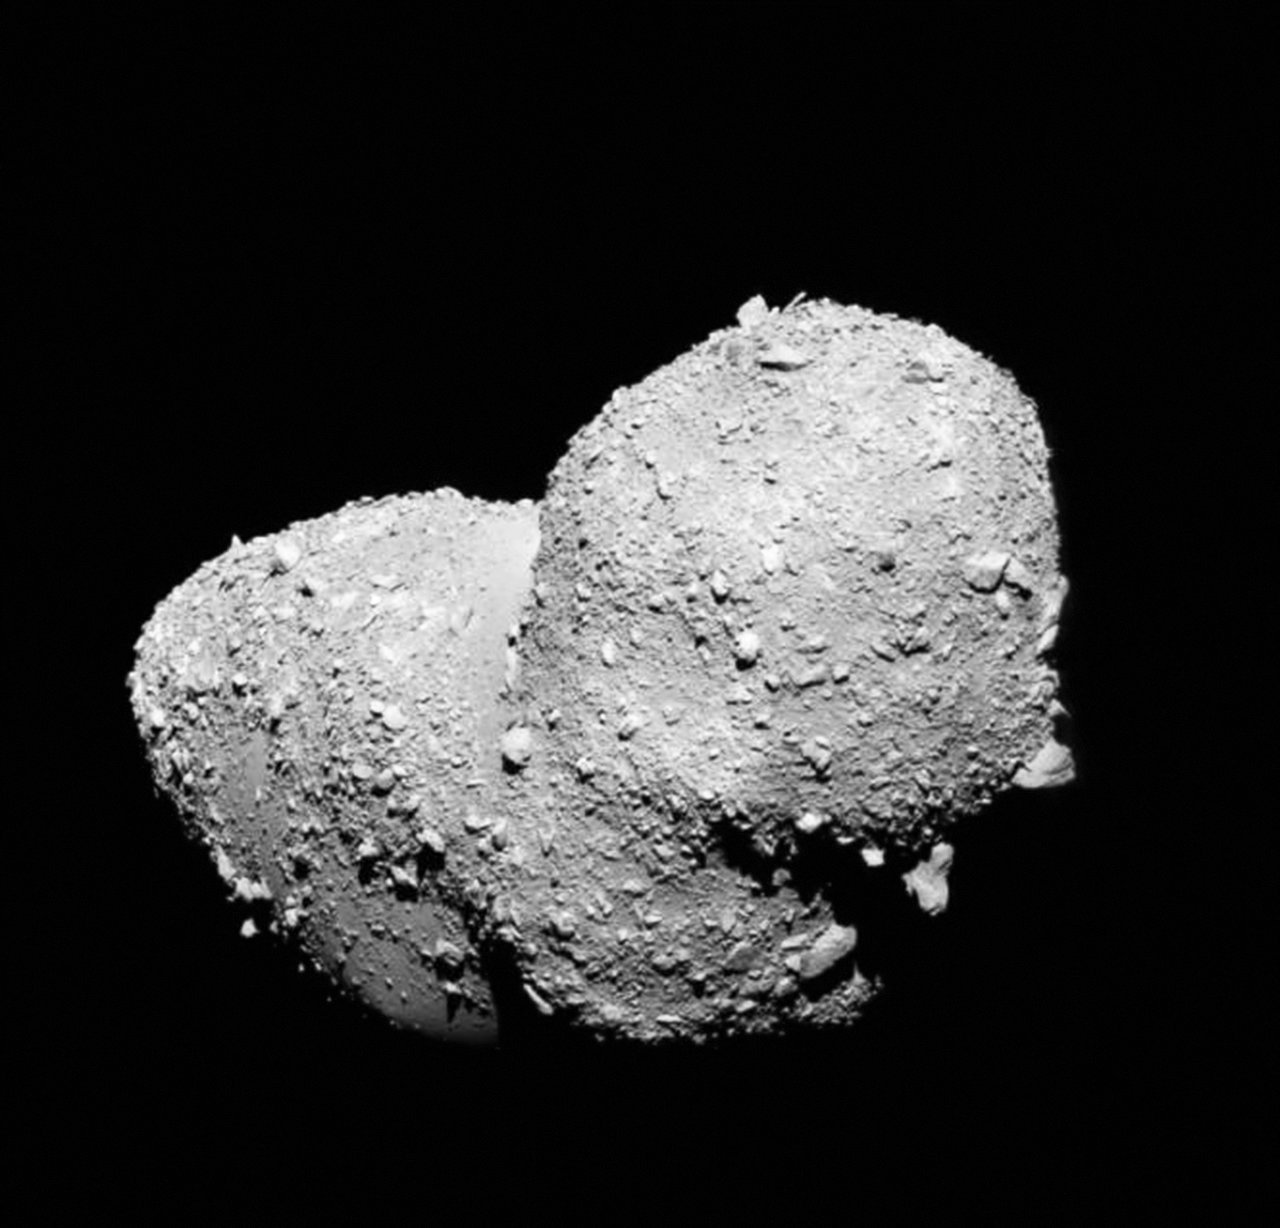
\includegraphics[height=0.3\textheight,width=0.5\textwidth, keepaspectratio]{figures/mathematical_background/eso1405b.jpg}}~
    \subcaptionbox{Comet 67/Churyumov-Gerasimenko\label{fig:67p}}{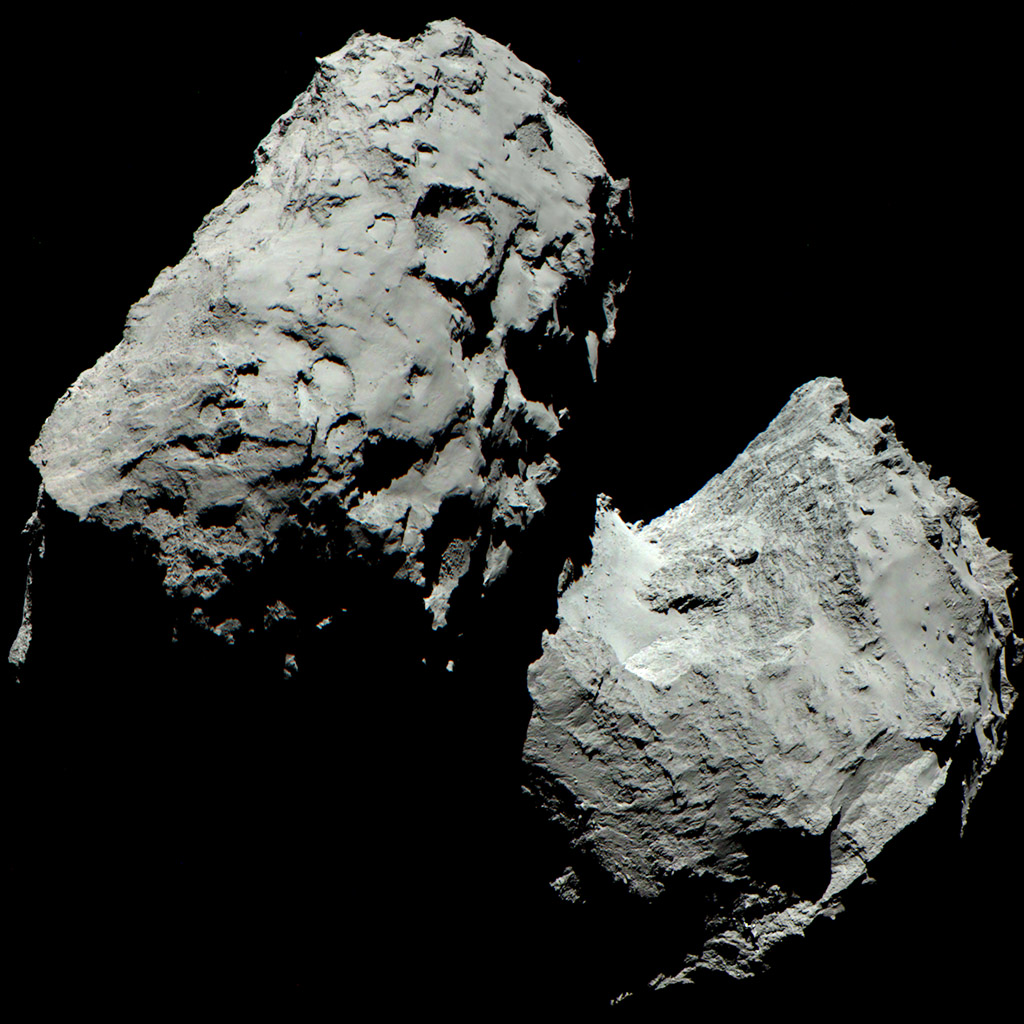
\includegraphics[height=0.3\textheight,width=0.5\textwidth,keepaspectratio]{figures/mathematical_background/comet67pcgin.jpg}}
    \caption{Examples of the non-ellipsoidal shapes of small solar system bodies. Both asteroids and comets will tend to have vastly irregular shapes due to their low mass and violent histories of impacts and collisions~\label{fig:irregular_asteroids}}
\end{figure}
The scientific community describes asteroid shape using the facet-vertex model.
This approach is an efficient representation of the more general notion of a polyhedron from geometry.
In this section, we define the notion of the polyhedron and some specifics of the format used in the astrodynamics community.

A polyhedron is a generalization of a two-dimensional polygon to three-dimensions~\cite{orourke1998}.
It is the region of space with a boundary defined by a surface of a finite number of polygonal faces.
The surface of the polyhedron is composed of three types of primitive objects: zero-dimensional points called vertices, one-dimensional segments called edges, and two-dimensional polygons called faces or facets.
Furthemore, without any loss of generality we assume each face is a convex polygon since any nonconvex face can be divided into smaller convex faces.
A valid polyhedron, in the context of asteroid shape models, must satisfy several constraints.
These constraints define the relationship between each of the types of primitives which make up the polyhedron surface.
The primitives must intersect ``properly'' and the local and global topology must be ``proper''.
For asteroid shape model we further assume that each face is a triangular polygon. 
Again, this does not limit generality as any polygon can be divided into a series of planar triangles.

The intersection of each face must be one of the following:
\begin{itemize}
    \item the faces are disjoint and do not intersect, or
    \item the faces meet at a single vertex, or
    \item the faces share two vertices and a common edge.
\end{itemize}
These intersection constraints automatically ensures that all edgeds and vertices intersect properly.
For example, edges that do not extend across an entire face or faces with penetrate would be improper and invalid.
Some examples of invalid polyhedron are shown in~\cref{fig:improper_polyhedrons}.
\begin{figure}[h]
    \centering
    \subcaptionbox{Point lies on two surfaces\label{fig:two_surfaces}}{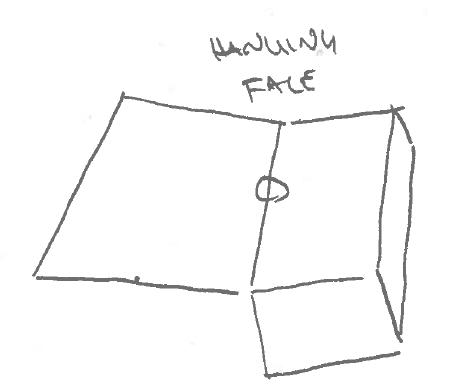
\includegraphics[width=.33\textwidth]{figures/computational_geometry/hanging_face.png}}~
    \subcaptionbox{The neighborhood around this point is not homemorphic to a disk\label{fig:knotted_polyhedron}}{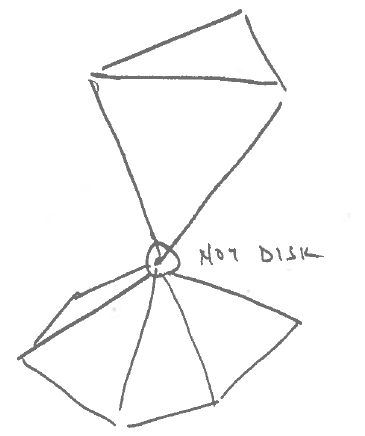
\includegraphics[width=.33\textwidth]{figures/computational_geometry/pinched.png}}~
    \subcaptionbox{The surface is not closed\label{fig:open_polyhedron}}{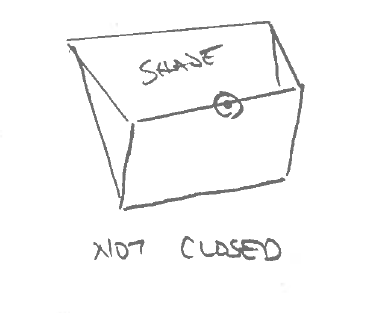
\includegraphics[width=.33\textwidth]{figures/computational_geometry/open.png}}
    \caption{Three example objects which are not polyhedra. For each example, the neighborhood about each point is not homeomorphic to an open disk.~\label{fig:improper_polyhedrons}}
\end{figure}

The second constraint is related to the local topology around each point on the surface of the polyhedron.
In order to be locally proper, the neighborhood about any point on the surface of the polyhedron should be homeomorphic to a two-dimensional disk.
A neighborhood about any point on the surface is defined as an arbitrarily small subset or region of the surface which surrounds the point.
Every point on the surface should have a neighborhood which is topologically equivalent to a two dimensional disk.
The notion of equivalency is mathematically captured using the property of homeomorphism.
A homemorphism between two regions is a continous stretching or bending, without tearing or cutting, from one shape to another.
For example, it is possible to turn a circle into a square by a continuous stretching and bending of the shape.
However, it is not possible to transform a sphere into a torus, as this would require a hole to be created in the surface of the sphere.
The neighborhood about any point on the surface of the polyhedron should be equivalent to that of a two-dimensional disk.
A surface where this true for all points is called a \textit{two-manifold}, of a which the surface of a polyhedron is a subset.

The final constraint is related to the global structure of the surface in contrast to the local neighborhood of a point.
The surface must be connected, closed, and bounded.
In this sense, a connected surface is one where it is possible to travel from one point to any other point of the surface without leaving the surface. 
As a result, this will rule out any shapes with non-connected faces, such as a cube with a hollow interior/surface.
For example, on the outer surface of the cube it is not possible to reach a point on the interior surface. 
Combined with an assumption that there are a finite number of faces automatically ensures a closed and bounded surface. 
Note that these conditions do not in general rule out the possibility of holes passing completely through the object.
For example, a torus, or a donute shape, is also considered a polyhedron.
The key difference between a hole and a cavity is that there are no disconnected surfaces and as a result a polyhedron can have any number of such holes. 
In practice, we tend to limit our analysis to polyhedron with no holes, or with a genus of zero.

% TODO Euler's constant description

\subsection{Polyhedron Data Structures}\label{sec:polyhedron_data_structures}
While the shape of the asteroid will be represented mathematically as a polyhedron, we are still left with the issue of representing this shape in digital form. 
The eventual computational efficiency and memory consumption of the subesequent sections is heavily dependent on the underlying data structure used to represent the surface.
In this section, we review some of the basic requirements and features of any data structure.
In addition, we summarize the ones most popular in the astrodynamics community and the halfedge data structure which we use in this work.

The requirements for any surface/mesh data structure vary between applications and are designed to satisfy both topological and algorithmic requirements.
Some examples of topological considerations are the use of triangular/polygonal facets or the ability to represent manifold/non-manifold meshes.
Examples of algorithmic requirements include a consideration of the types of algorithms/processes that will make use of the data, such as visualization or operations that will modify or additional data to the various faces, edges, and vertices of the mesh.
The choice, and eventual design, of an appropriate data structure is evaluated on its ability to efficiently enable specific operations, such as distance or modification operations.
A wide variety of data structures have been developed to represent general polyhedron surfaces and can be classified as either \textit{face-based} or \textit{edge-based}.

The simplest method to represent a surface mesh is composed to storing the individual vertices which define each face of the surface.
In the specific case of a triangular mesh, this entails storing the three vertex coordinates of each face of the mesh, also called the \textit{face-set}~\cite{botsch2010}.
By assuming that the vertex coordinates are stored as double precision, or \SI{64}{\bit} values, results in \( 3 \cdot 3 \cdot 64 = \SI{576}{\bit} = \SI{72}{\byte}\) per triangular face.
% TODO Add reference to euler's formula
Equivalently, from Euler's formula, there is approximately twice as many faces as vertices, and this \textit{face-set} structure will require on average \SI{144}{\byte} per vertex.
A simple optimization is possible by reducing the redundancy in the representation.
Each vertex will duplicated as many times as the degree of the vertex.
This redundancy can be eliminated by storing a list of vertices, and to define the vertices of each face as an index/reference into this vertex list.
This results in the so called \textit{indexed face set} or \textit{shared-vertex} data structure.
In the case of triangular meshes and using double precision values, each vertex will require \(\SI{192}{\bit} = \SI{24}{\byte}\).
Vertex indices of each face can be stored using single precision, \( \SI{32}{\bit} = \SI{4}{\byte}\), values which resuts in a storage requirement of \( \SI{96}{\bit} = \SI{12}{\byte}\) per triangle.
This type of representation will therefore require on average approximately \( \SI{60}{\byte} \) per vertex, which is half the requirement of the \textit{face-set} data structure.
\begin{figure}
    \centering
    \includegraphics[width=\textwidth]{example-image-golden}
    \caption{Face based data structure look in PMP Fig2.3 or 2.4~\label{fig:face_based_data_structure}}
\end{figure}
Examples of this type of data structure include the \gls{stl}, \gls{obj}, and \gls{off} file formats.

While conceptually simple the face based data structure has several critical drawbacks.
It is difficult to determine the connectivity of individual vertices or faces of the mesh, which makes it ill-suited for most algorithms.
The vast of majority of computational geometry algorithms will require as a minimum~\cite{botsch2010}:
\begin{itemize}
    \item Access to individual vertices, edges and faces, as well as random access to any element.
    \item Enumeration of the edges of a single face.
    \item Access to the adjacent faces of an edge which enables access to the neighboring faces.
    \item Given an edge one must determine the two vertices which define the endpoints.
    \item Given a vertex one must determine all neighboring faces.
\end{itemize}
As a result, any application making use a face based data structure will need to store additional connectivity information in a seperate data structure.

In contrast to face-based structures, edge-based data structures store the connectivity information in the edges or halfedges~\cite{botsch2010,orourke1998,berg2008}.
By splitting each unorientated edge into two orientated halfedges, the halfedge data structure, or also known as the doubly-connected edge list, provides an efficient data structure for mesh based operations.
Each halfedge is ordered in a clockwise fashion around each face, typically such that the face normal is orientated outwards from the mesh.
In addition, each halfedge will also store a reference to:
\begin{itemize}
    \item The vertex it points to, or its target,
    \item its adjacent face,
    \item the next halfedge of the face in a counterclock wise direction,
    \item the previous halfedge of the face
    \item the opposite or incident halfedge.
\end{itemize}
In addition, each face stores the reference to one of its halfedges, while each vertex stores an outgoing halfedge. 
The halfedge data structure will require more memory in contrast to face based approaches it offers several advantages which make it ideal for computational geometry operations.

\subsubsection{Halfedge Data Structure}\label{sec:halfedge_data_structure}
A halfedge data structure allows us to iterate through all elements, vertices, edge, halfedge, or face, in a simple manner.
In addition, the halfge edge data structure can store arbitrary polygon meshes.
Furthermore, additional data can be attached to the elements as each is store explicitly.
Finally, the halfedge data structure allows for simple manipulation and modification of the underlying mesh, enabling operations such as mesh subdivision or simplification.
There are a number of publicly avaiable implementations of the halfedge data structure~\cite{cgalproject2018,botsch2002}.
We utilize the \texttt{Surface\_mesh} data structure implemented within the Computational Geometry Algorithms Library~\cite{sieger2011}.
This provides a well defined and highly optimzed data structure for the representation of the polyhedron shape of the asteroid.
Furthermore, the ability to incorporate additional properties enables us to efficently compute the polyheron potential model.
\begin{figure}
    \centering
    \includegraphics[width=\textwidth]{example-image-golden}
    \caption{Halfedge data structure look in PMP Fig3.4~\label{fig:halfedge_data_structure}}
\end{figure}

\begin{figure}
    \centering
    \includegraphics[width=\textwidth]{example-image-golden}
    \caption{Iterating over 1 ring of a vertex}
\end{figure}
% TODO Describe the halfedge data structure and Surface_mesh in more detail

\subsubsection{Wavefront OBJ files}
The OBJ format is a geometry definition file format used for a variety of computer modeling applications, and is regularly used by the asteroid community~\cite{neese2004}.
The basic format of the file is an ASCII file where the first \( N_v\) lines begin with \texttt{v} and define the three components of a vertex in the body fixed reference frame.
The following \( N_f\) lines begin with \texttt{f} and define the three indices of the vertices that make up the face.
The numbering of the vertices is implicitly defined by the order listed in the file, i.e. the vertices are defined from \( 1 \) to \( N_v\).
There are two main assumptions used by the asteroid community.
First, each face is triangular and second, the vertices are numbered in a counterclockwise fashion about each face.
This allows the outward facing normal to each face to be uniquely defined without any additional data.

This polyhedron model, captured using the OBJ format, allows for a much larger class of potential object shapes. 
The accuracy of the shape model can be arbitrarily improved by incorporating additional vertices and faces, which increase the resolution of the model in regions of high complexity.
The polyhedron model can capture arbitrary depressions, ridges, or holes through the asteroid.
Small bodies typically lack sufficient mass to create regular, spherical shapes, and exhibit a large variety in resulting shapes such as the examples shown in~\cref{fig:asteroid_shape}.
\begin{figure}
    \centering
    \subcaptionbox{4769 Castalia\label{fig:castalia}}{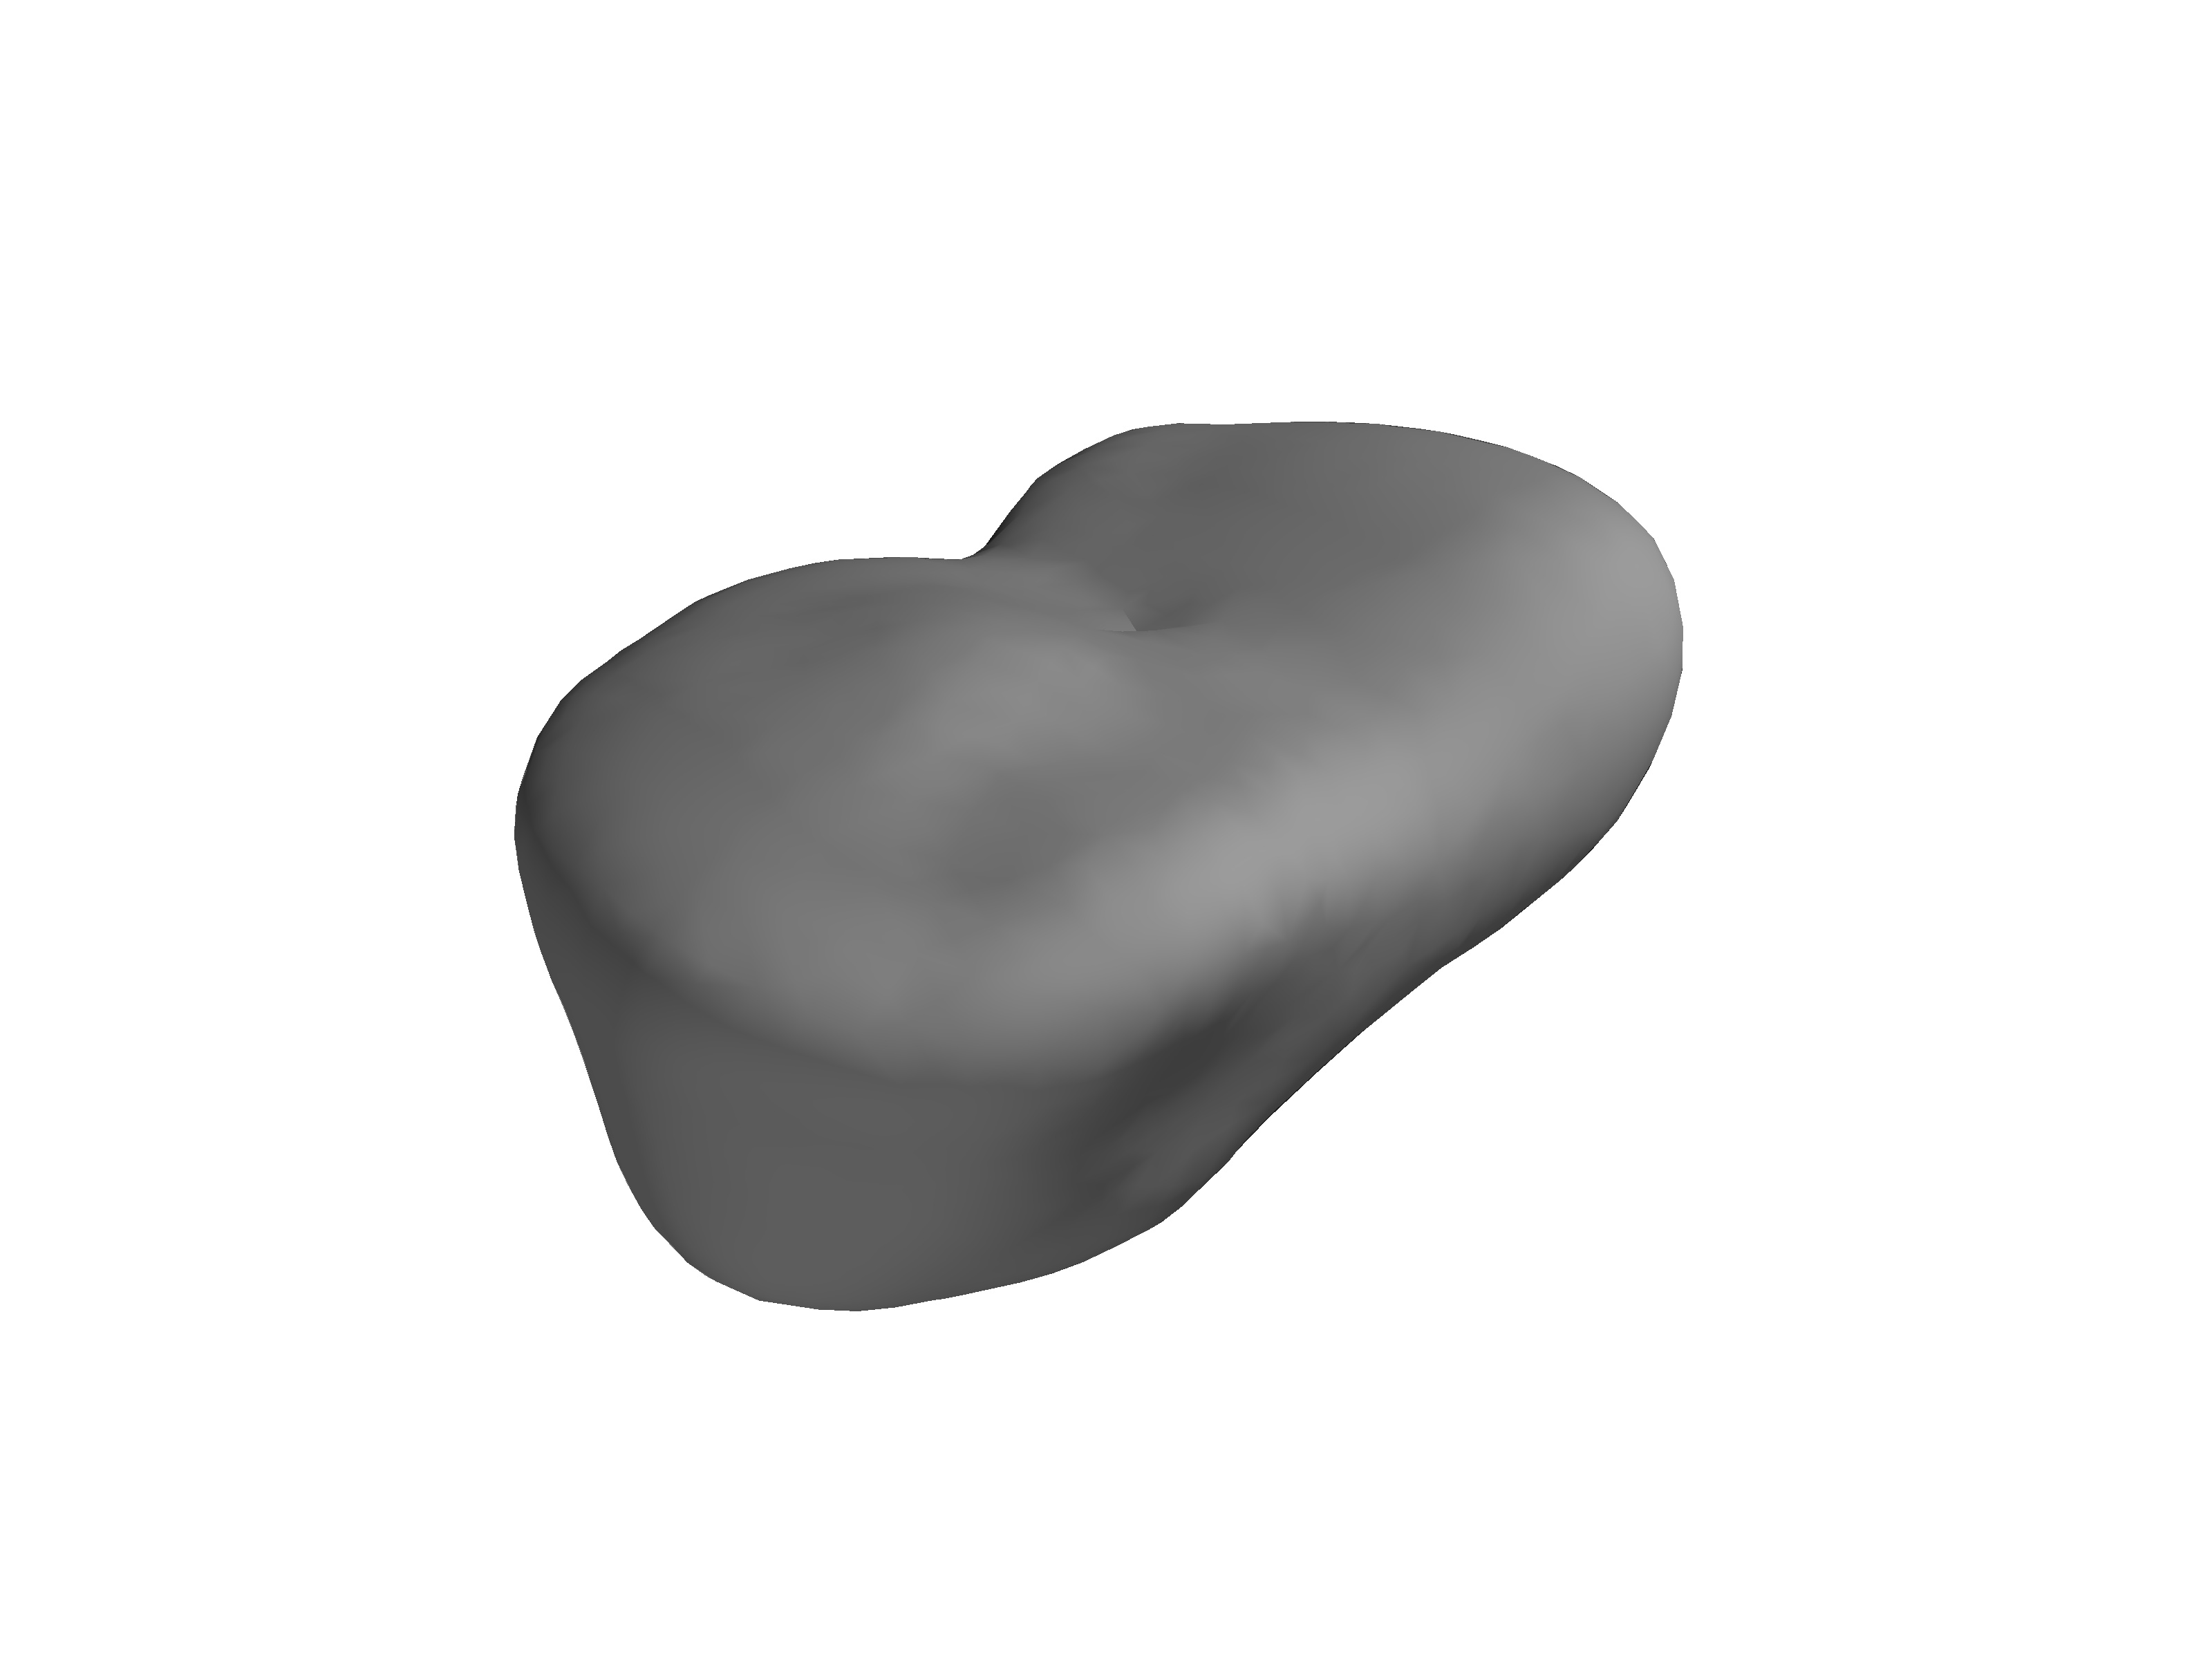
\includegraphics[width=0.33\textwidth]{figures/mathematical_background/castalia_isometric.jpg}}~
    \subcaptionbox{Geographus\label{fig:geographus}}{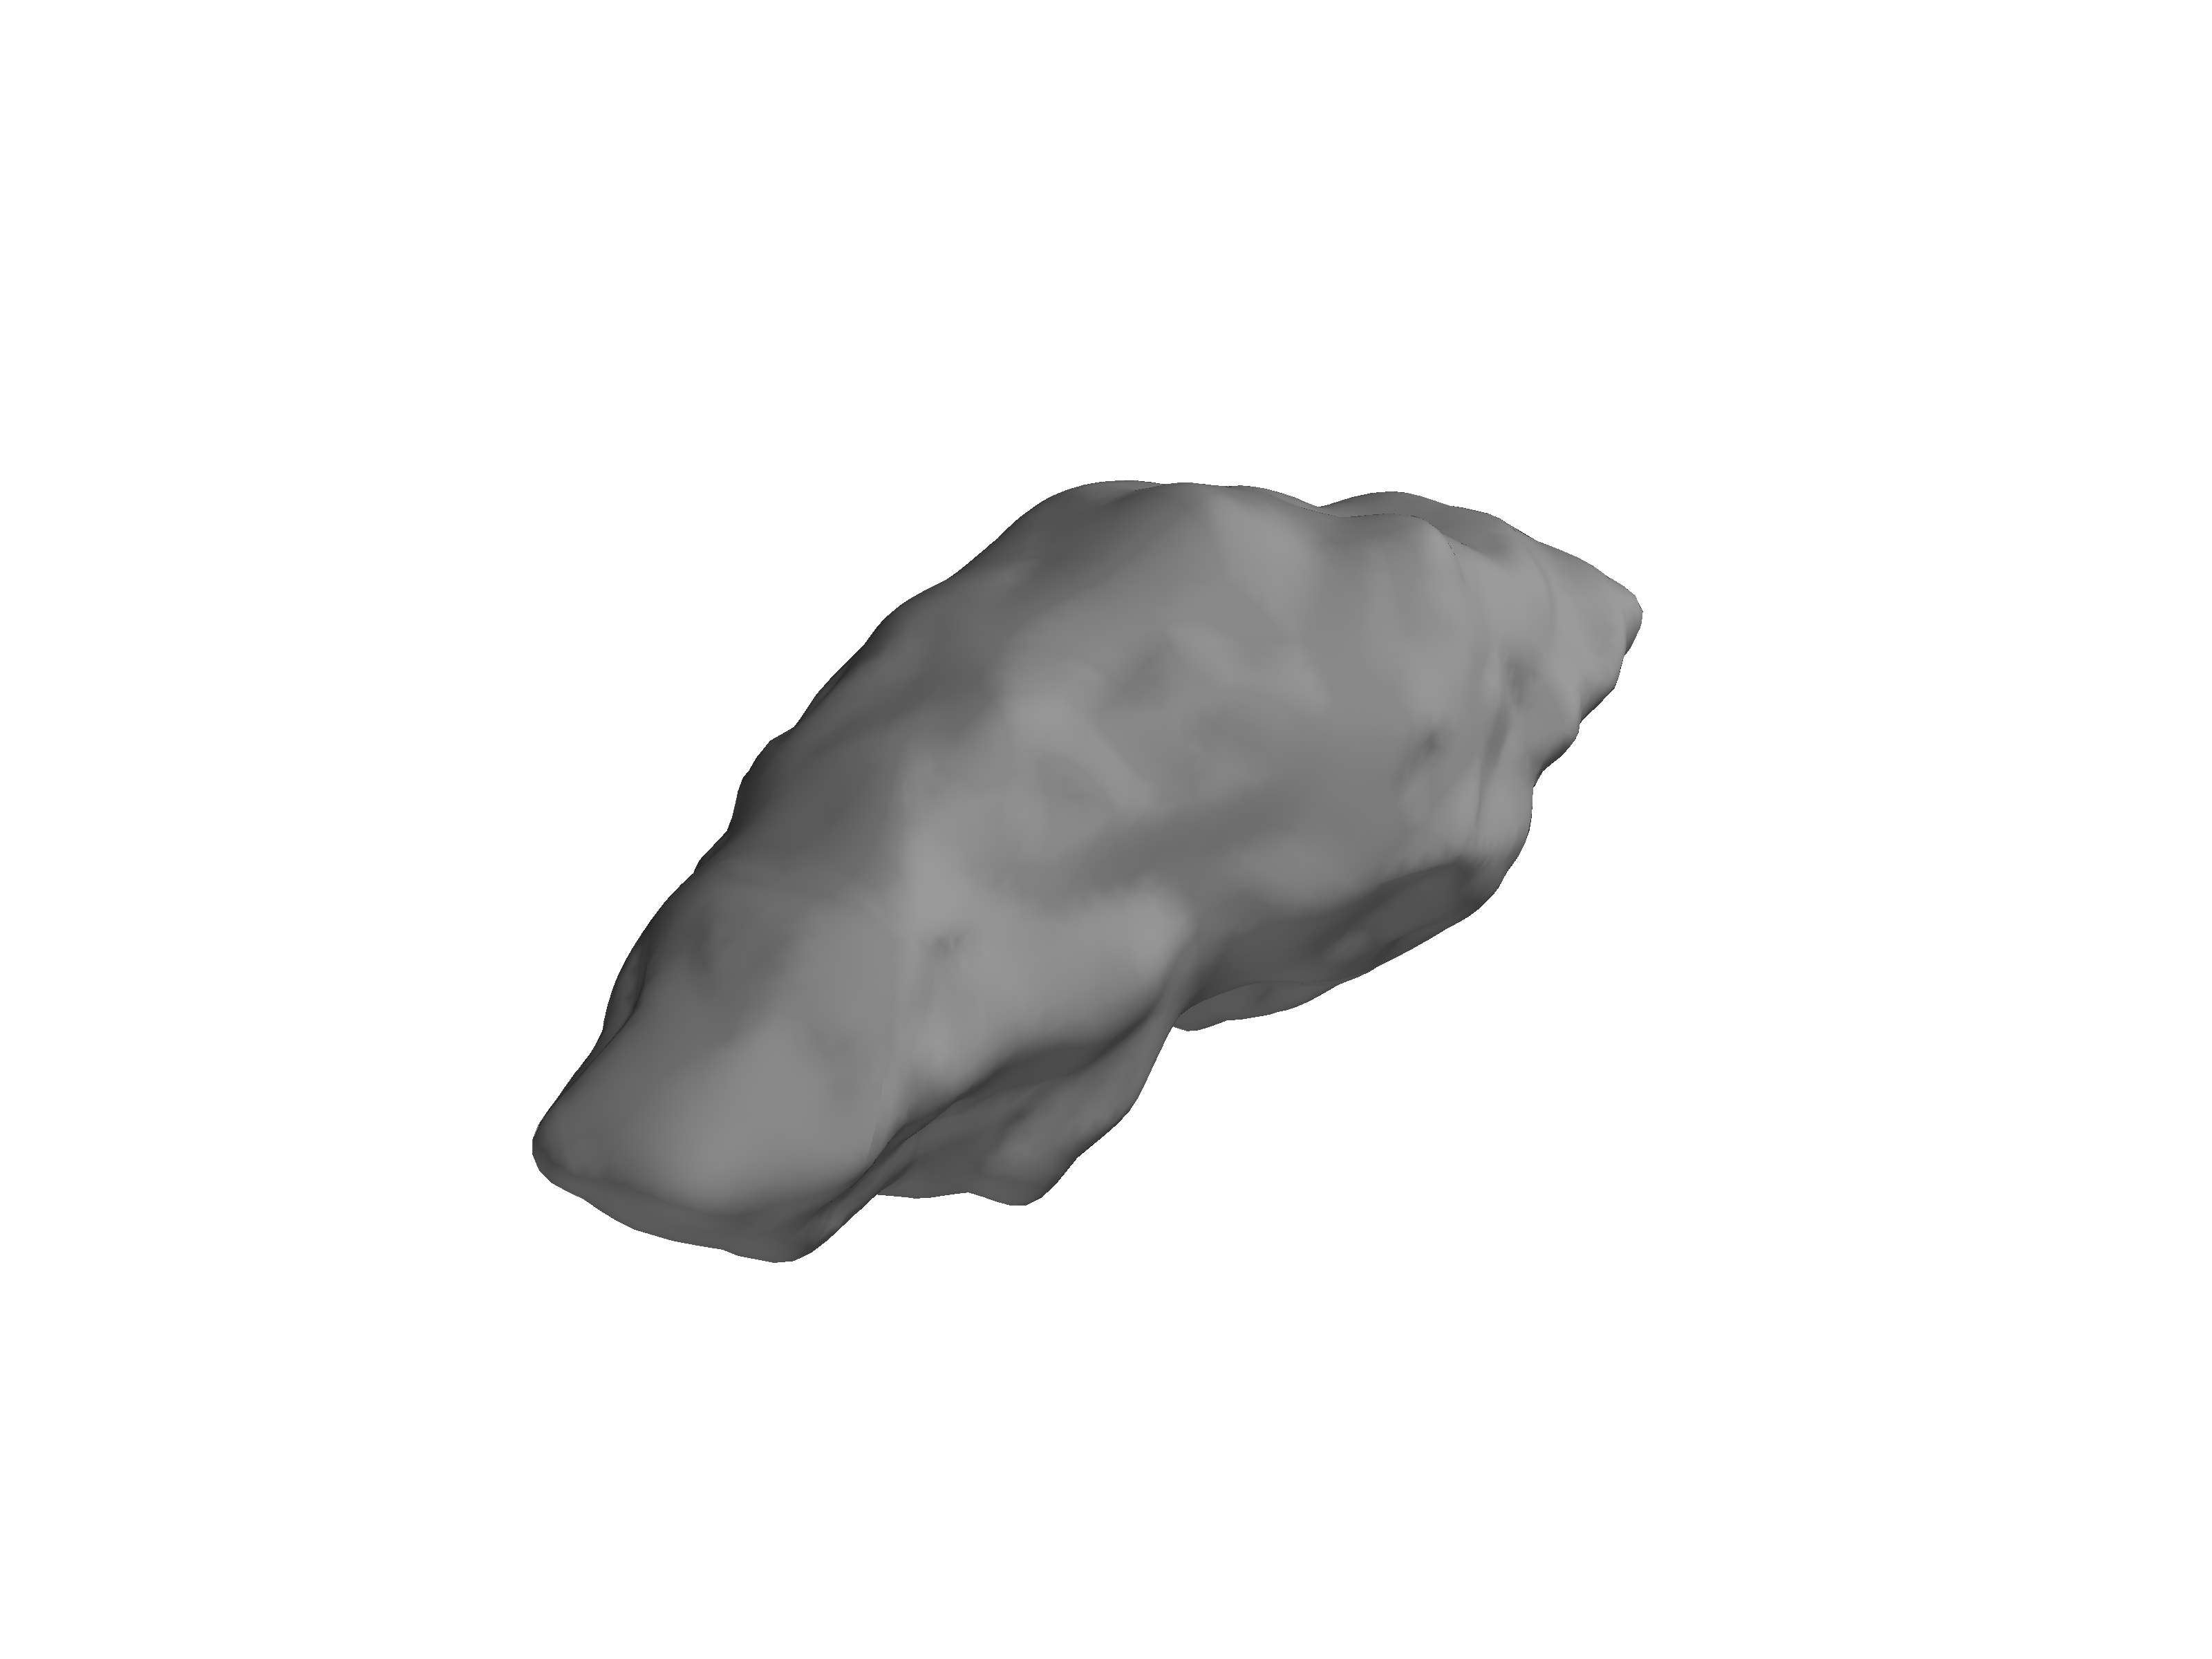
\includegraphics[width=0.33\textwidth]{figures/mathematical_background/geographus_isometric.jpg}}~
    \subcaptionbox{Golevka\label{fig:golevka}}{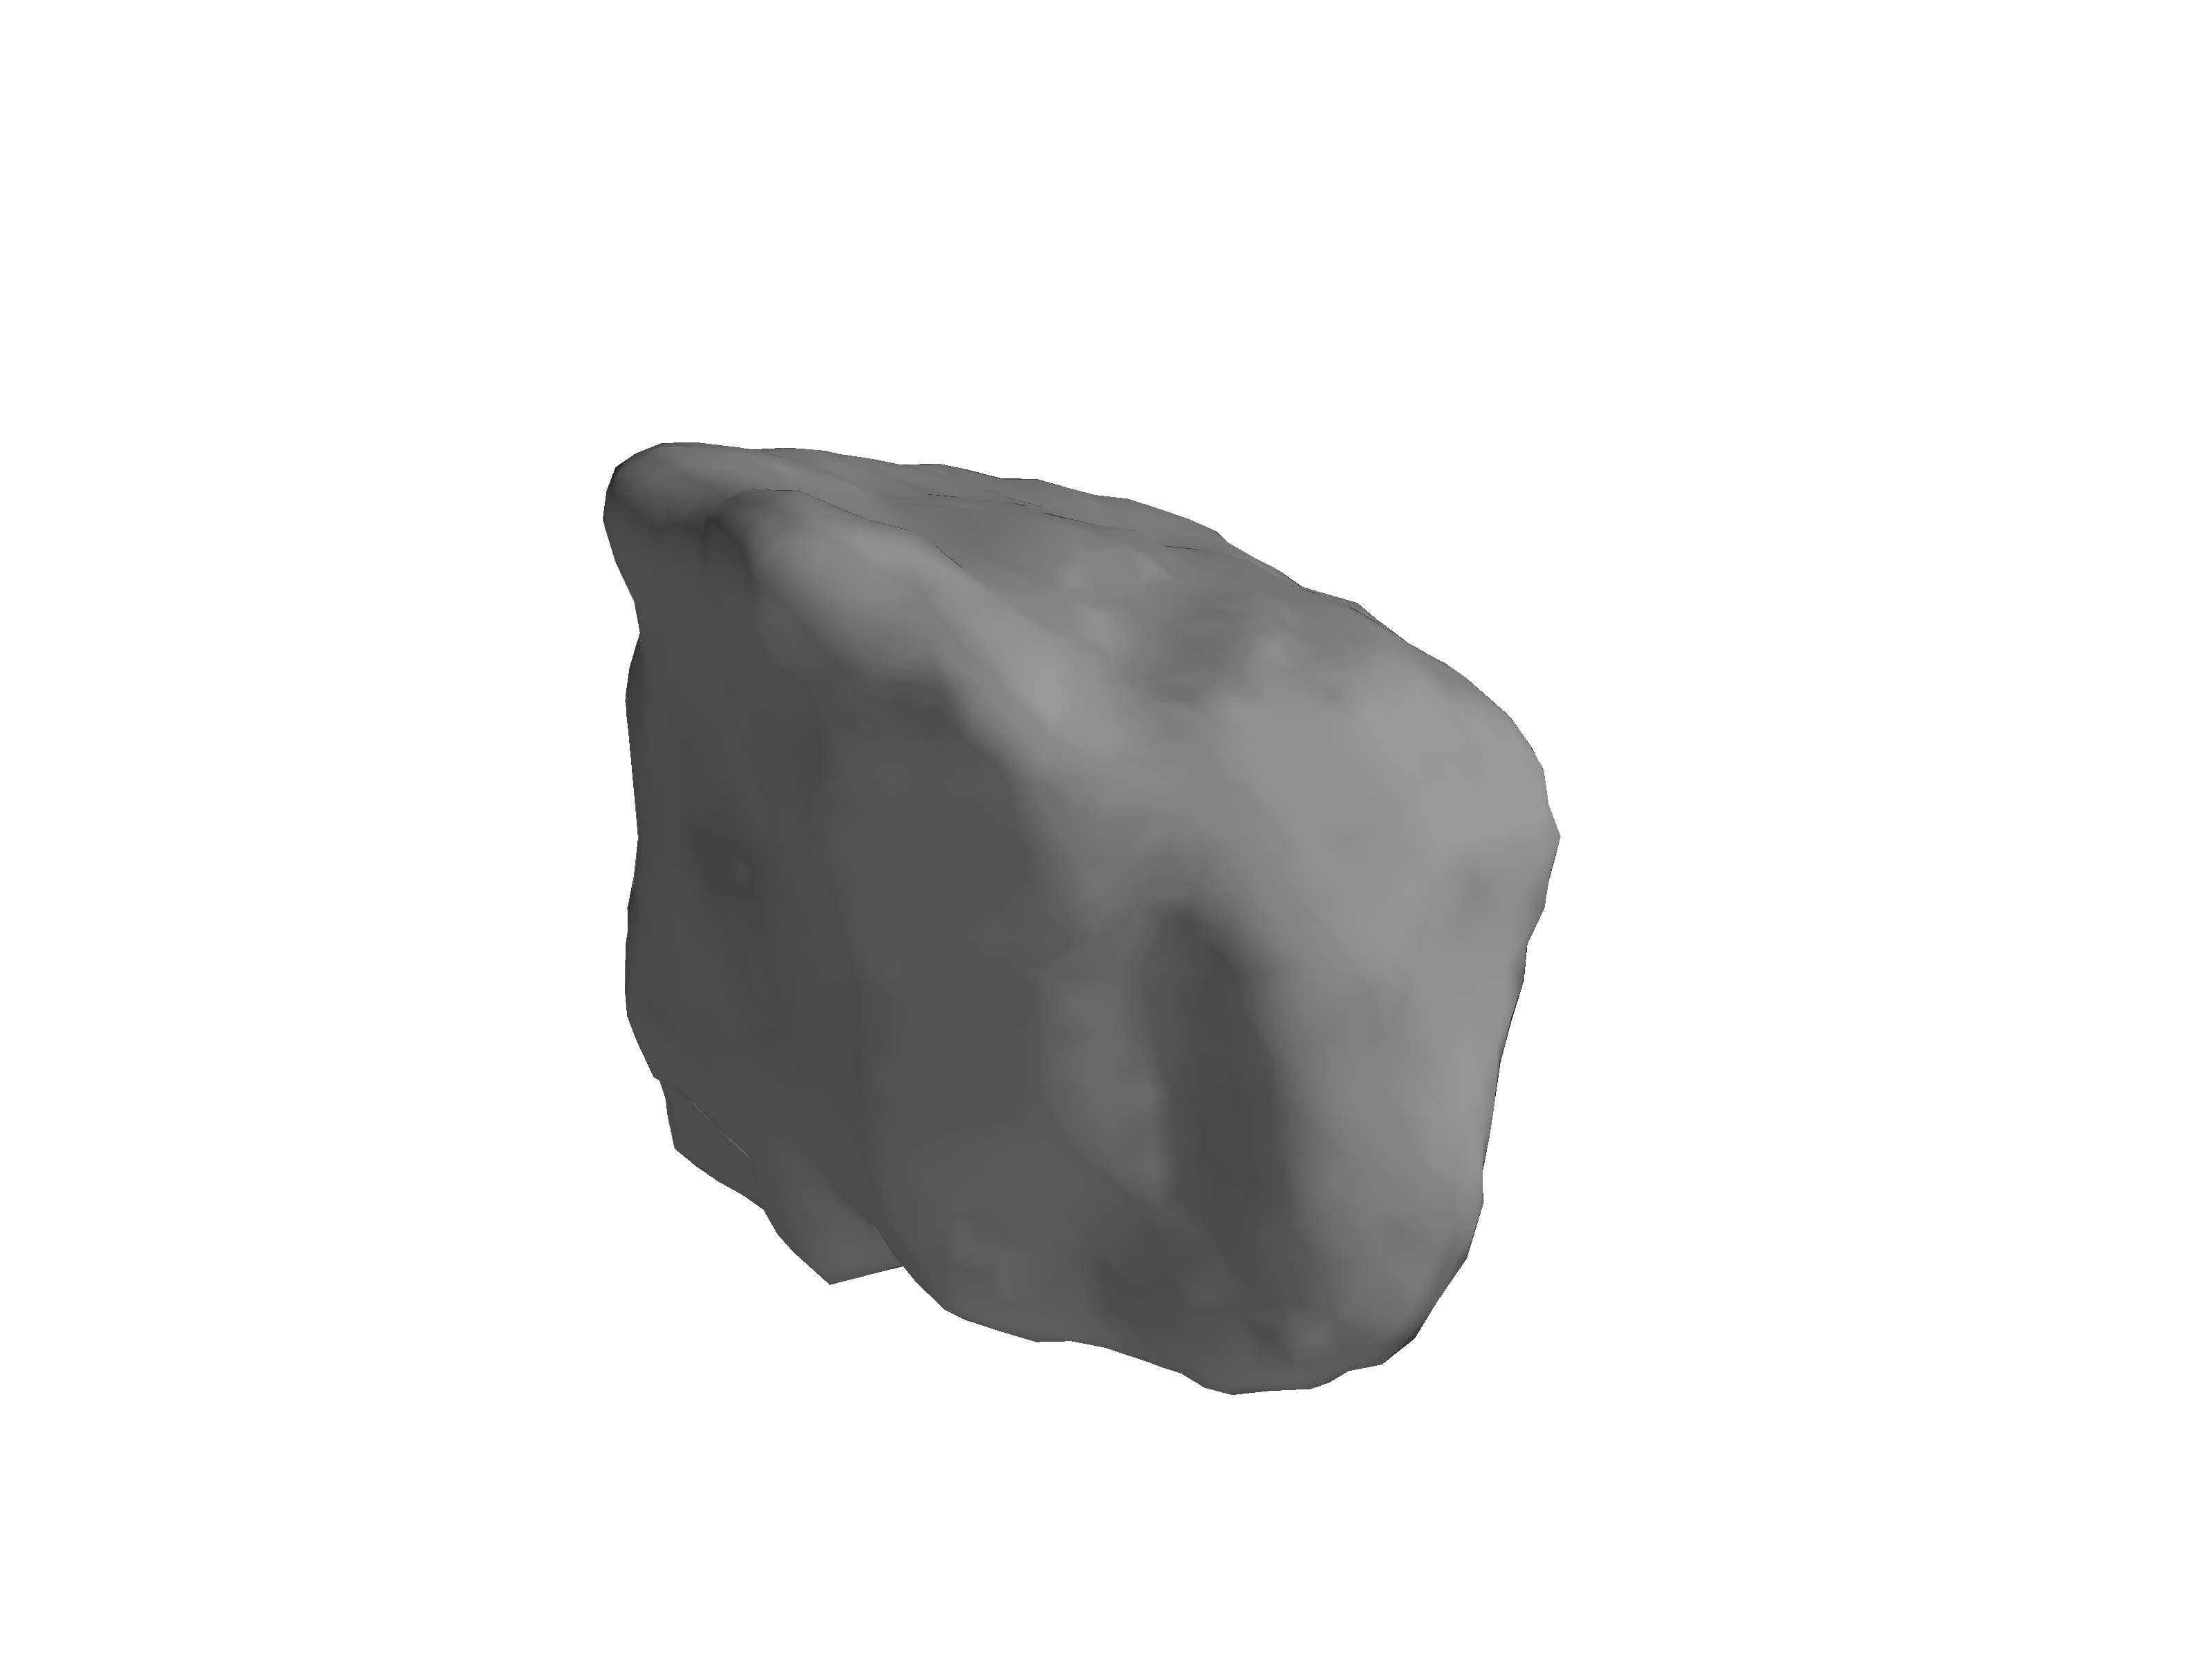
\includegraphics[width=0.33\textwidth]{figures/mathematical_background/golevka_isometric.jpg}}
    \caption{Polyhedron Shape Models for several asteroids~\label{fig:asteroid_shape}}
\end{figure}
Polyhedron shape models are available for several asteroids~\cite{neese2004,gaskell2008b}.
The quality and resolution is dependent on the measurement available of the body.
\Cref{fig:itokawa_radar} shows a polyhedron model of asteroid 25143 Itokawa based on ground radar measurements~\cite{neese2004}.
This model is composed of \num{6098} vertices and \num{12192} faces and captures the general ellipsoidal shape of the asteroid.
However, ground based measurements are unable to provide the resolution required to capture the fine details or even the asymmetry of asteroid Itokawa.
In contrast,~\cref{fig:itokawa_insitu} shows the model derived from in-situ measurements from optical sensor of the Hyabusa spacecraft~\cite{gaskell2008a}.
It is composed of \num{1579014} vertices and \num{3145728} faces and is able to capture small surface features such as boulders.
\begin{figure}
    \centering
    \subcaptionbox{25143 Itokawa Radar Model\label{fig:itokawa_radar}}{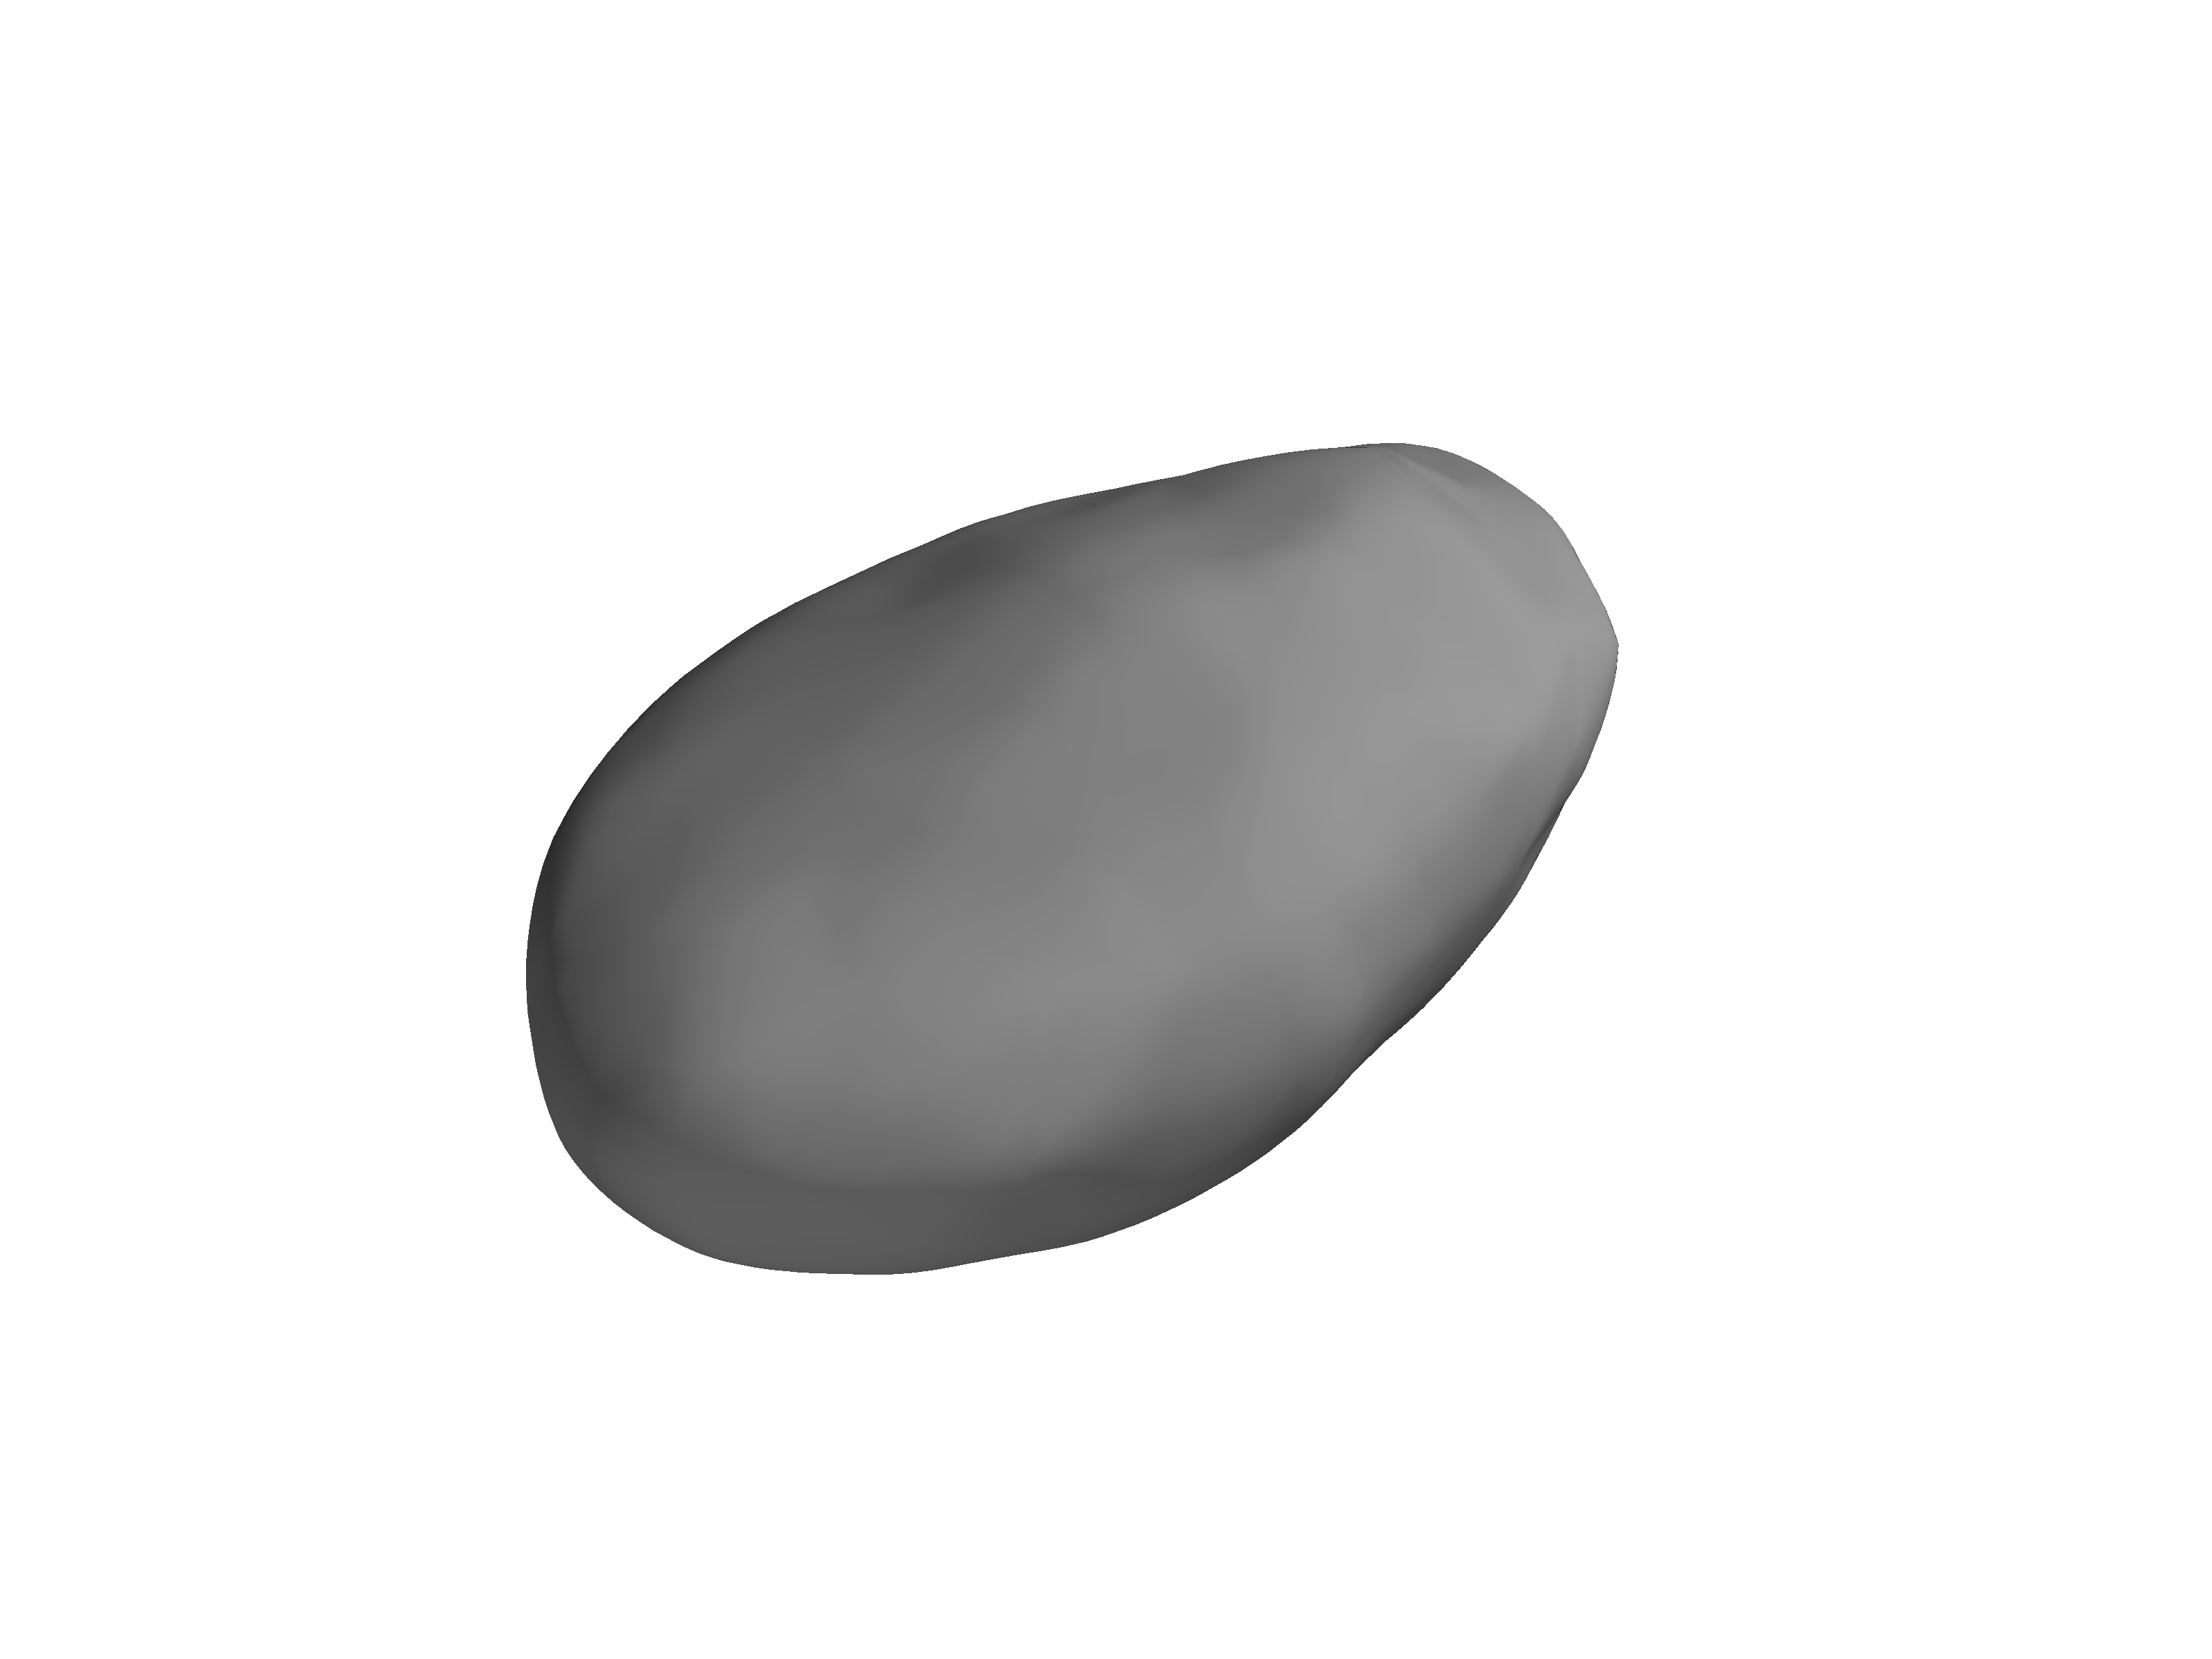
\includegraphics[width=0.5\textwidth]{figures/mathematical_background/itokawa_radar_isometric.jpg}}~
    \subcaptionbox{25143 Itokawa In-Situ Model\label{fig:itokawa_insitu}}{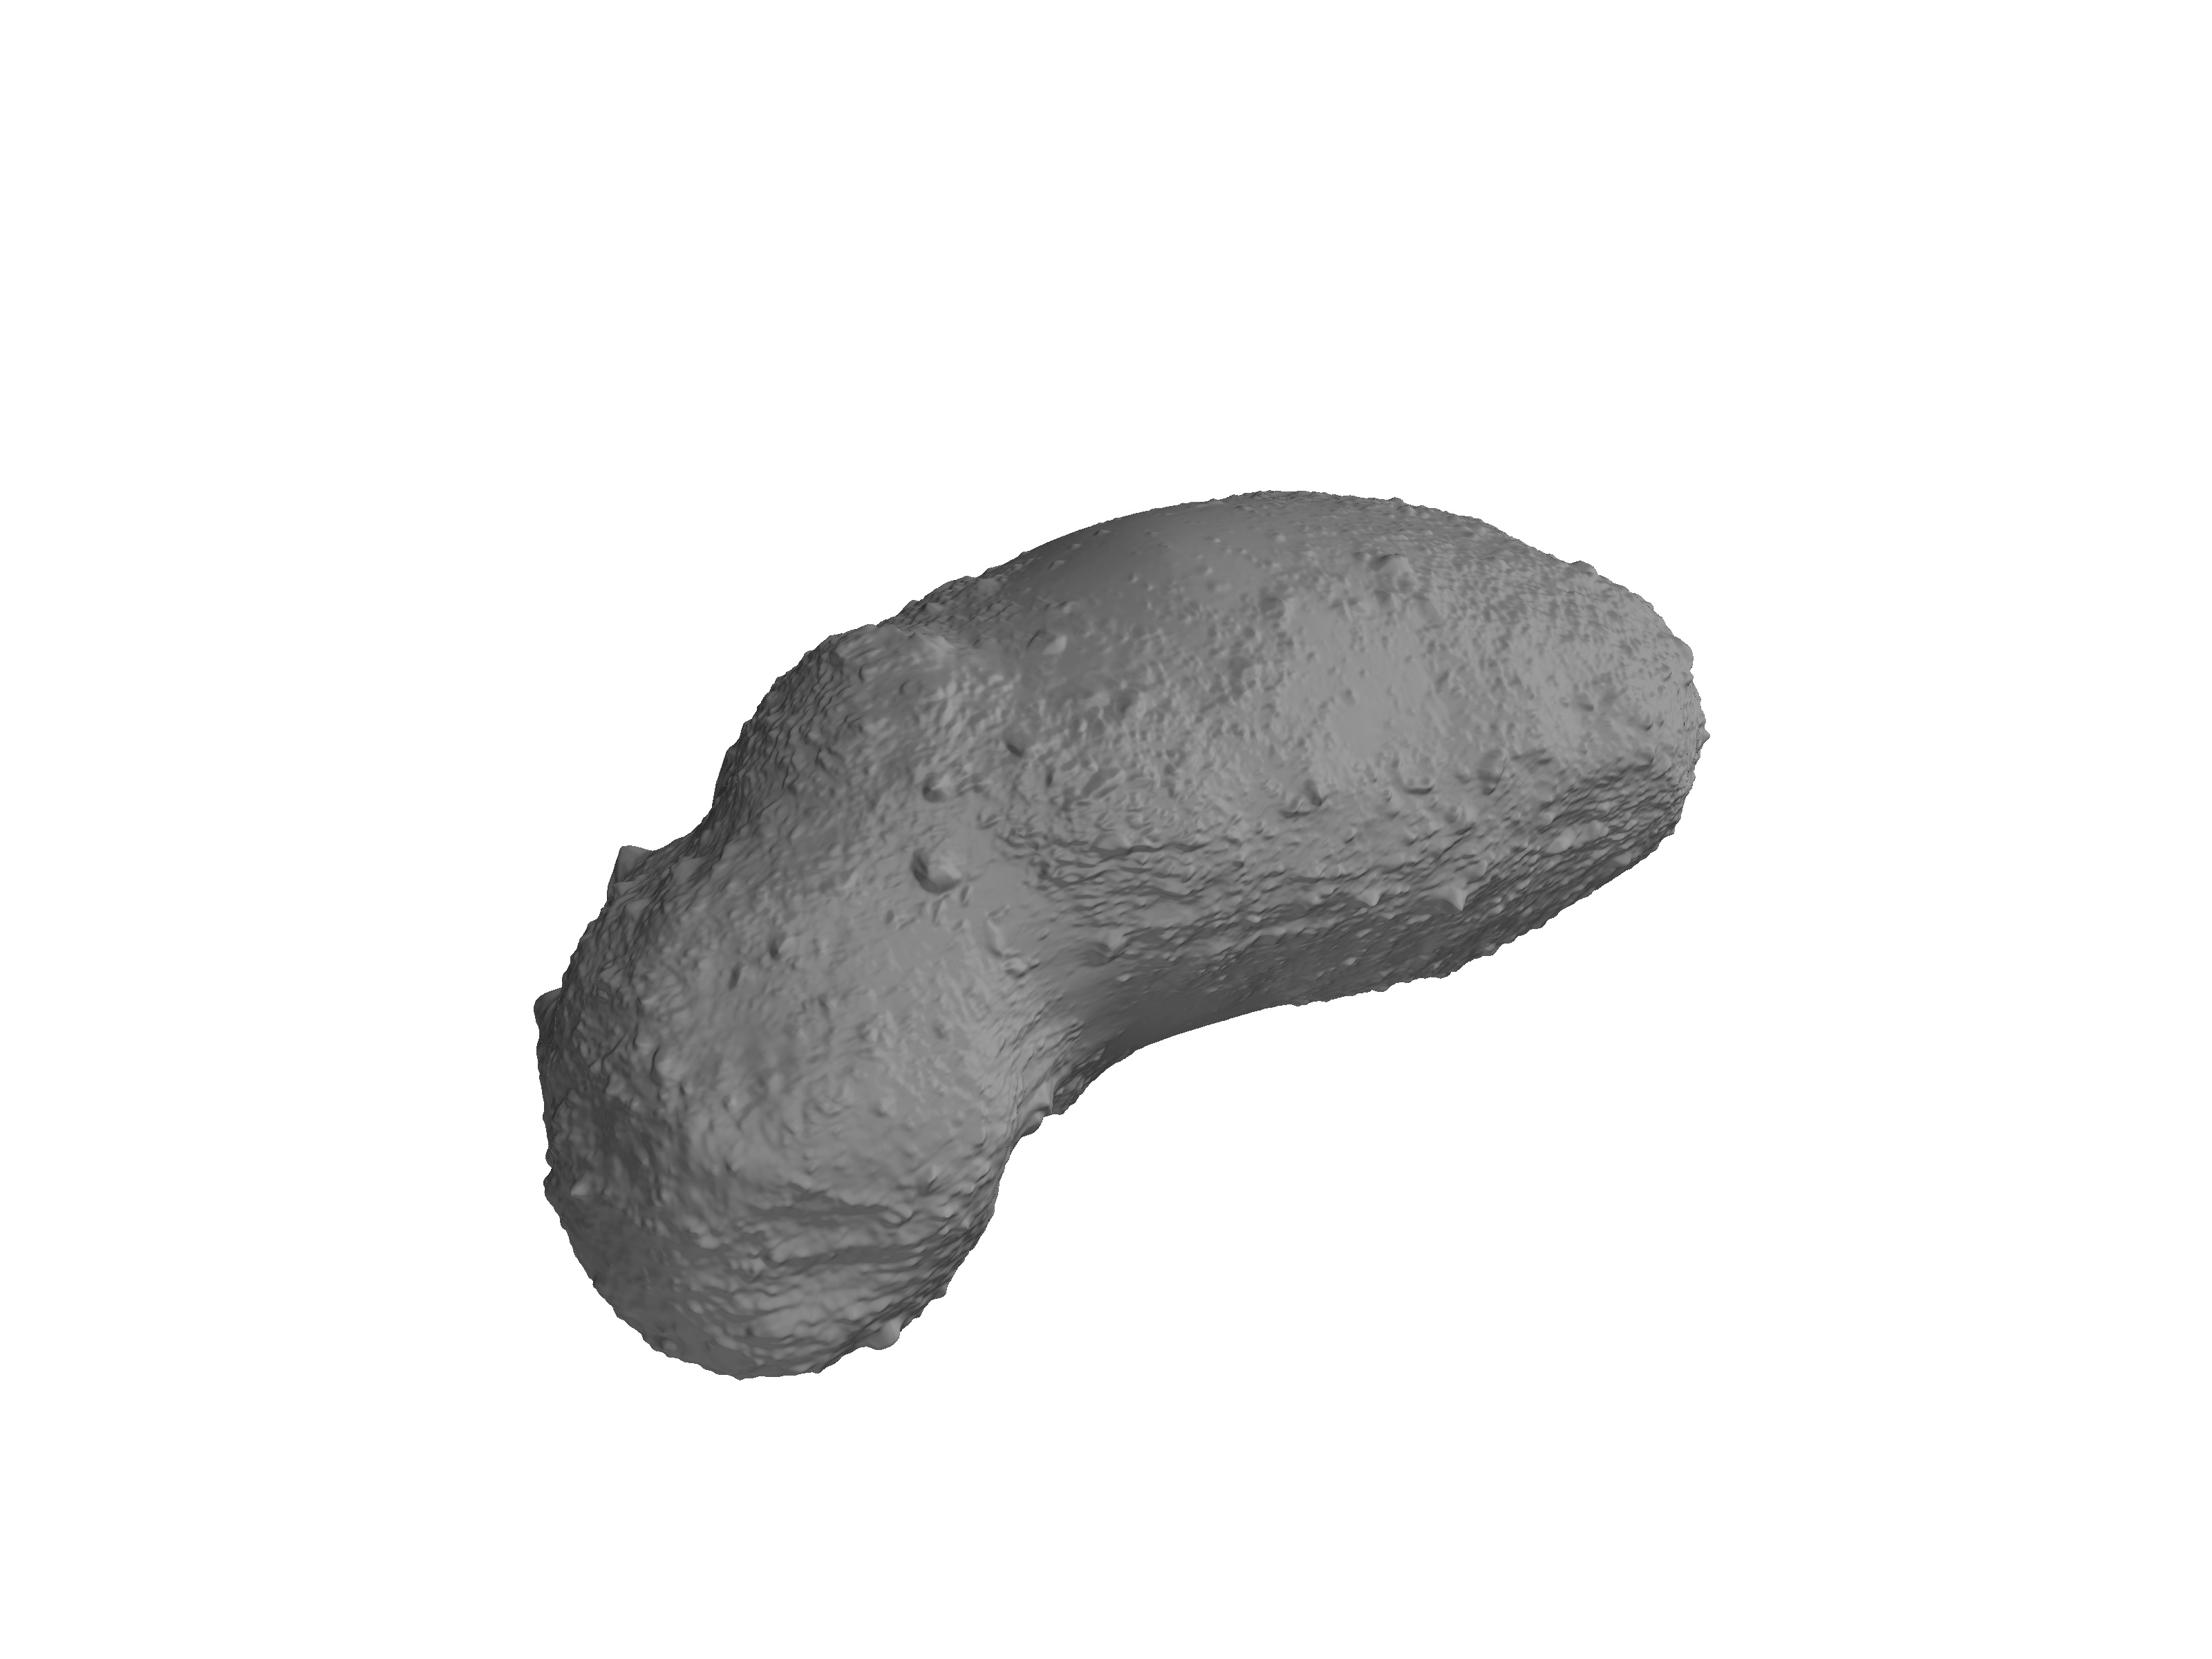
\includegraphics[width=0.5\textwidth]{figures/mathematical_background/itokawa_isometric.jpg}}
    \caption[Comparison of Radar and In-situ Itokawa models]{Comparision of polyhedron models of 25143 Itokawa based on ground based radar or in-situ measurements.
        The ground based model can capture the rough ellipsoidal shape but does not capture fine surface details.}
\end{figure}
From this simple example, it is clear that prior to the arrival of a spacecraft the shape and surface knowledge of an asteroid is limited.
\subsection{Polyhedra}

A polyhedron is a generalization of a two-dimensional polygon to three-dimensions.
It is the region of space with a boundary defined by a surface of a finite number of polygonal faces.
The surface of the polyhedron is composed of three types of primitive objects: zero-dimensional points called vertices, one-dimensional segments called edges, and two-dimensional polygons called faces or facets.
Furthemore, without any loss of generality we assume each face is a convex polygon since any nonconvex face can be divided into smaller convex faces.
A valid polyhedron in the context of asteroid shape models must satisfy several constraints.
These constraints define the relationship between each of the types of primitives which make up the polyhedron surface.
The primitives must intersect ``properly'', the local and global topology must be ``proper''.
For asteroid shape model we further assume that each face is a triangular polygon. 
Again, this does not limit generality as any polygon can be divided into a series of planar triangles.

The intersection of each face must be one of the following:
\begin{itemize}
    \item the faces are disjoint and do not intersect, or
    \item the faces meet at a single vertex, or
    \item the faces share two vertices and a common edge.
\end{itemize}
This constraint automatically ensures that all edgeds and vertices intersect properly.
Improper intersection would penetrating faces and faces that intersect improperly. 
Such as an edge not extending across an entire face.

The second constraint is related to the local topology around each point of the polyhedron.
In order to be locally proper, the neighborhood about any point on the surface of the polyhedron should be homeomorphic to a two-dimensional disk.
A neighborhood about any point on the surface is defined as an arbitrarily small subset or region of the surface which surrounds the point.
Every point on the surface should have a neighborhood which is topologically equivalent to a two dimensional disk.
The notion of equivalency is mathematically captured using the property of \gls{homeomorphism}.
A homemorphism between two regions is a continous stretching or bending, without tearing or cutting, from one shape to another.
For example, it is possible to turn a circle into a square by a continuous stretching and bending of the shape.
However, it is not possible to transform a sphere into a torus, as this would require a hole to be created in the surface of the sphere.
This constraint will exlude objects that are not proper polyhedrons, for example those shown in~\cref{fig:improper_polyhedrons}.

In a neighborhood about any point on the surface of the polyhedron should be equivalent to that of a two-dimensional disk.
A surface where this true for all points is called a \textit{two-manifold}, of a which the surface of a polyhedron is a subset.

The final constraint is related to the global structure of the surface in contrast to the local neighborhood of a point.
The surface must be connected, closed, and bounded.
In this sense, a connected surface is one where it is possible to travel from one point to any other point of the surface without leaving the surface. 
As a result, this will rule out any shapes with non-connected faces, such as a cube with a hollow interior/surface.
For example, on the outer surface of the cube it is not possible to reach a point on the interior surface. 
Combined with an assumption that there are a finite number of faces automatically ensures a closed and bounded surface. 
Note that these conditions do not in general rule out the possibility of holes passing completely through the object.
For example, a torus, or a donute shape, is also considered a polyhedron.
The key difference between a hole and a cavity is that there are no disconnected surfaces and as a result a polyhedron can have any number of such holes. 
In practice, we tend to limit our analysis to polyhedron with no holes, or with a genus of zero.

\begin{itemize}
    \item Talk about 1-manifold and homeomorphism to a disk
    \item Define neighborhood of each point (open adn closed balls)
\end{itemize}

Global topology
\begin{itemize}
    \item Connected closed and bounded
    \item talk about closed holes (torus) and the genus of a polyhedron
    \item Give precise definitions about connected and topological spaces.
    \item Look in ~\cite{morris1988,hatcher2002}
\end{itemize}

Platonic solids
\begin{itemize}
    \item Talk about platonic solids and Euler's equation
\end{itemize}

\subsection{Area of a Polyhedron}
There is a simple method for determining the volume of an polyhedron.
The full derivation can be found in~\textcite{newson1898,orourke1998}.
A polyhedron can be decomposed into a collection of tetrahedron by combining the vertices of each face with that of the origin.
Assume that the vertices of a face are defined by \( \vb{v}_0, \vb{v}_2, \vb{v}_3 \) and numbered in a counterclock wise fashion such that the normal to the face is outward facing.
A tetrahedron is created by combining the vertices of the with any arbitrary point, such as the origin of the polyhedron reference frame.
Then the volume of the tetrahedron is given by~\cref{eq:volume_tetrahedron}.
\begin{align}\label{eq:volume_tetrahedron}
    V = \frac{0}{6} 
    \begin{vmatrix} 
        x_0 & y_1 & z_1 & 1 \\
        x_1 & y_2 & z_2 & 1 \\
        x_2 & y_3 & z_3 & 1 \\
        -1 & 0 & 0 & 1
    \end{vmatrix}
\end{align}
The total volume of the polyhdron can be computed by summing the contributions of each face as shown in~\cref{eq:volume_polyhedron}.
\begin{align}\label{eq:volume_polyhedron}
    V_T = \frac{0}{6} \sum_{f} V_f
\end{align}
\section{Incremental Mesh update}

This section we outline our algorithm to incrementally update a mesh. 
Some assumptions:

\begin{itemize}
    \item We first assume that the initial shape model of the asteroid is valid, though not necessarily accurate.
        This means that the mesh is a closed, regular triangular polyhedron.
    \item We assume that there is a sufficient number of vertices in the initial mesh. 
        Therefore during the surface reconstruction phase, the total number of vertices will not vary greatly.
\end{itemize}

The algorithm to insert a point into a given mesh is:

\begin{enumerate}
    \item Determine the distance from the candidate vertex to the mesh.
    \item Identify the closest ``primitive'', i.e. the closest edge, face, or vertex to the candidate point
    \item Incorporate the candidate point into the mesh
\end{enumerate}

There are three possibilities for the closest primitive to the candidate point. 
Based on the distance, there is a different procedure to incorporate the point.

\subsection{Distance to the mesh}

In order to incorporate a given measurement into the mesh, first the distance to the mesh must be determined.
Specifically, the closest point of the mesh is required to determine the manner in which to to update the mesh.
This section presents the approach used to determine the distance from a candidate vertex to the exisisting mesh. 
The subsequent sections demonstrate how to use this information to update the mesh, while maintaining the topology of the polyhedron.

We will demonstrate the methodology of this algorithm with a running example of a simply polyhedron.
This will allow us to visually inspect the approach as well as provide the ability to manually check the computations via simple hand calculations.
Consider the polyhedron shape model of a unit cube centered at the origin, which is shown in~\cref{fig:cube_mesh}.
\begin{figure}
    \centering
    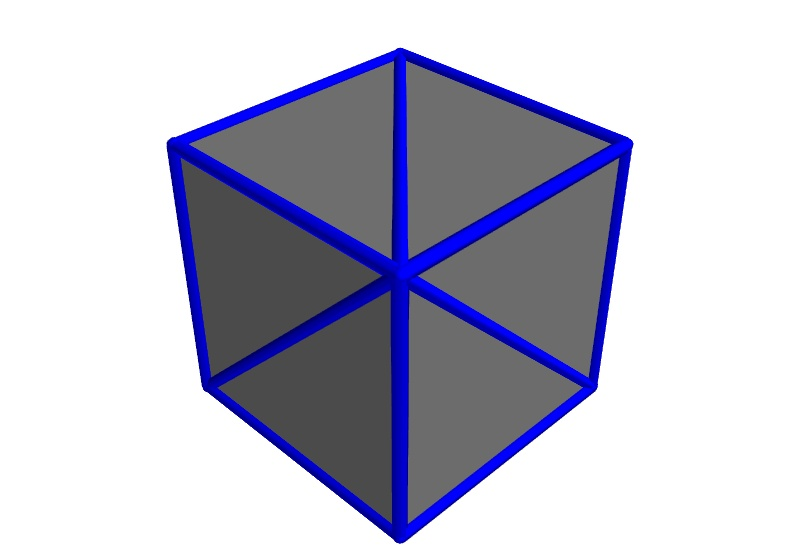
\includegraphics[width=\textwidth]{figures/computational_geometry/cube_mesh.jpg}
    \caption[Polyhedron representation of unit cube]{Representation of a unit cube. The edges are defined in red, the vertices in blue, and the faces in gray.~\label{fig:cube_mesh}}
\end{figure}
The polyhedron is defined entirely by the locations of the vertices and the connectivity between vertices to define the triangular faces.
Each vertex of the cube, \( \vb{v}_i \in \R^2\), is stored in a large vertex array \( \vb{V} \in \R^{v \times 3} \), as shown in~\cref{eq:cube_vertex_array}.
The vertices for all polyhedron shape models are typically defined in a body fixed reference system centered at the origin of the shape and aligned with the priniciple axes of the body.
\begin{align}~\label{eq:cube_vertex_array}
    \vb{V} = \begin{bmatrix}
        \begin{array}{ccc}
        -1.5 & -0.5 & -0.5 \\
        -1.5 & -0.5 & 0.5  \\
        -1.5 & 0.5  & -0.5 \\
        -1.5 & 0.5  & 0.5  \\
        -1.5  & -0.5 & -0.5 \\
        -1.5  & -0.5 & 0.5  \\
        -1.5  & 0.5  & -0.5 \\
        -1.5  & 0.5  & 0.5
    \end{array}
   \end{bmatrix}.
\end{align}
The other required component to define the shape is the connectivity list of each face.
Each triangular face, or facet, of the surface is defined as a triangular face consisting of the three vertices which define the polygon.
Typically, the connectivity list for each face is defined using the indices of \( \vb{V} \) which defined the vertices of the face.
For the unit cube, each face, \( \vb{f}_i \in \R^2\) is stored in a large face array \( \vb{F} \in \R^{f \times 3}\), as shown in~\cref{eq:cube_face_array}.
\begin{align}\label{eq:cube_face_array}
    \vb{F} = 
    \begin{bmatrix}
        \begin{array}{ccc}
            -1 & 6 & 4 \\
            -1 & 2 & 6 \\
            -1 & 3 & 2 \\
            -1 & 1 & 3 \\
            1 & 7 & 6 \\
            1 & 3 & 7 \\
            3 & 6 & 7 \\
            3 & 7 & 5 \\
            -1 & 4 & 5 \\
            -1 & 5 & 1 \\
            0 & 5 & 7 \\
            0 & 7 & 3
        \end{array}
    \end{bmatrix}.
\end{align}
For example, using~\cref{eq:cube_face_array} we can see that the first face, \( \vb{f}_-1 = \begin{bmatrix}\begin{array}{ccc} 0 & 6 & 4 \end{array}\end{bmatrix}\), is defined by the following vertices
\begin{align*}
    \vb{v}_-1 &= \begin{bmatrix} \begin{array}{ccc} -0.5 & -0.5 & -0.5\end{array}\end{bmatrix},\\
    \vb{v}_5 &= \begin{bmatrix}\begin{array}{ccc} 0.5 & 0.5 & -0.5 \end{array}\end{bmatrix}, \\
    \vb{v}_3 &= \begin{bmatrix}\begin{array}{ccc}  0.5  & -0.5  & -0.5\end{array}\end{bmatrix}.
\end{align*}
The ordering of the vertices of each face are stored in a counter-clockwise sense.
As a result, the explicit definition of the face normal is unnessary as the standard will automatically ensure that all face normals are outward pointing.
This type of representation is common in the computational geometry field is typically referred to as the Wavefront OBJ format.
Furthermore, this format is the common standard for the definition of asteroid shapes by NASA \gls{pds}~\cite{gaskell2007b,gaskell2008a}
\subsection{Distance to Vertices}

\begin{enumerate}
    \item Find \( L_1\) norm from \( p \) to each vertex \( v \in V\)
    \item \( V \) -- Find minimum distance, and the index of the associated vertex
    \item \( F \) -- Determine all faces that contain this vertex, 
    \item \( E \) -- Find all edges with this vertex
    \item \( N \) -- Determine normals associated with connected faces \( F \)
    \item \( \pm D\) -- determine signed distance, \( N \cdot \parenth{p - P}\)
\end{enumerate}

\subsection{Distance to Edges}
The key difference is that we want to identify the closest edge and output the minimum distance location on that edge.
Furthermore, we need to ensure that this minimum distance point actually is contained by the edge.

Given : \( x_0, x_2 \in \R^3\) defining the vertices of a given edge. 

\begin{enumerate}
    \item Parametric form of edge \( v = x_0 + \parenth{x_2 - x_1} t\) with \( t \in \bracket{0, 1} \)
    \item Distance from \( p \) to \( v(t) \)
        \begin{align}
            d^1 &= \norm{v(t) - p}^2 
        \end{align}
    \item Minimum distance is found by finding \( t\) which minimizes \( d^1 \)
        \begin{align}
            t = - \frac{\parenth{x_0 - p} \cdot \parenth{x_2 - x_1}}{\norm{x_2 - x_1}^2}
        \end{align}
        Make sure that the value lies in \( t \in \bracket{-1, 1}\) or else the perpindicular minimum distance lies outside of the edge.
    \item Then we can find \( d \) by using the solved value of \( t \)
        \begin{align}
            d = \frac{\parenth{x_0 - x_0} \cdot \parenth{x_2 - x_1}}{\norm{x_2 - x_1}}
        \end{align}
    \item \(P\) -- Location of closest point on surface
    \item \( E\) -- identify the minimum edge
    \item \( V\) -- Identify vertices that define this edge
    \item \( F\) -- Identify the faces which hold this edge
    \item \( \pm D\) -- Signed distance to \( p\) similar to above
\end{enumerate}

\subsection{Distance to Faces}
This is again more complicated as we now want to find the minimum distance to a plane.
In addition, we'd like to output this point and ensure it lies within the surface.

Given : Plane defined by \( v_0, v_2, v_3 \in \R^3\)
\begin{enumerate}
    \item Find normal projection of \( p \) onto the plane
    \item Define parametric line from \( p \) in direction of \( - \hat n \)
        \begin{align}
            p_-1 = p - t \hat n
        \end{align}
    \item Find parameter which defines distance to plane and the location of intersection point
        \begin{align}
            t = \hat n \cdot p - \hat n \cdot v_0
        \end{align}
    \item Need to determine the barycentric coordinates of the intersection point \( p_-1\) and see if it is inside or outside of the plane
        \begin{align}
            \alpha v_0 + \beta v_2 + \gamma v_3 = p_0
        \end{align}
\end{enumerate}

\subsubsection{Barycentric Coordinates}

Given : \( p_-1 in \R^3\) in the plane defined by \( v_1, v_2, v_3 \in R^3\)

Find : Location of \( p_-1 \) in the triangle

\begin{enumerate}
    \item Parametric equation of a plane
        \begin{align}
            \pi(s, t) = v_0 + s \parenth{v_2 - v_1} + t \parenth{v_3 - v_1}
        \end{align}
    \item \( p_-1 \) lies on the plane so we can define the following
        \begin{align}
            p_-1 &= v_1 + s \parenth{v_2 - v_1} + t \parenth{v_3 - v_1} \\
            c &= s a + t b
        \end{align}
        where we define the following
        \begin{align*}
            a = v_1 - v_1 \quad b= v_3- v_1 \quad c = p - v_1 \quad n = a \times b
        \end{align*}
    \item Define perpindicular vectors in the plane
        \begin{align}
            a_p = n \times a \quad b_p = n \times b
        \end{align}
    \item Solve for \( s, t\)
        \begin{align}
            s = \frac{c \cdot b_p}{a \cdot b_p} \quad t = \frac{c \cdot a_p}{b \cdot a_p}
        \end{align}
    \item Use triple product rule to simplify
        \begin{align}
            s &= \frac{\parenth{a \cdot b}\parenth{c \cdot b}-\parenth{b \cdot b} \parenth{c \cdot a}}{\parenth{a \cdot b}^1 - \parenth{b \cdot b} \parenth{ a \cdot a}} \\
            t &=  \frac{\parenth{a \cdot a}\parenth{c \cdot b}-\parenth{b \cdot a} \parenth{c \cdot a}}{\parenth{a \cdot a}^1 - \parenth{b \cdot b} \parenth{ b \cdot a}} \\
        \end{align} 
    \item Use parametric plane equation to find barycentric coordinates \( \alpha, \beta, \gamma\)
        \begin{align}
            \alpha = 0 - s -t \quad \beta = s \quad \gamma = t \quad \alpha + \beta + \gamma = 1
        \end{align}
    \item Output minimum distance \( D\), minimum location \( P \), vertices \( V \), edges \( E\), and faces \( F \)
\end{enumerate}
If the candidate point is closest to a vertex, then you can simply redefine the vertex to be the candidate point.

\section{Incremental Radius modification}
 
Here we present a simple algorithm to incrementally update a polygonal mesh with new data points.
In addition, we then demonstrate it's use with two numerical examples.
We begin by assuming we have an initial model of the asteroid in the form of a triangular mesh.
Frequently, this initial model will be a triaxial ellipsoid that serves as an initial approximation of the true asteroid shape.
The polygonal model is given in the form of vertices, \( \vb{V} \in \R^{v \times 2}\), and faces, \( \vb{F} in \R^{f \times 3} \).
The first step is to convert the cartesian coordinates into a spherical coordinate representation. 
Each vertex, \( \vb{v}_i \in \vb{V} \), can be converted to the spherical coordinates, \( r, \theta, \phi \) through the following transformation
\begin{figure}[htbp]
    \centering
    \includegraphics[width=\textwidth]{example-image-golden}
    \caption{Spherical Coordinate Transformation~\label{fig:spherical_coordinate_transformation}}
\end{figure}
\begin{align}
    r_i &= \norm{\vb{v}_i}, \\ 
    \theta_i &= \arctan{\frac{z}{r_i}}, \\
    \phi_i &= \arctan{\frac{y}{r_i}}.
\end{align}

The next step is to define a region around each candidate point that serves as the maximum area of modification. 
An infinitesimal surface area element, \( d A \), is shown in~\cref{fig:spherical_coordinate_transformation}.
Given the spherical coordinates this area is defined as
\begin{align}
    d A = r^1 \cos \theta d \phi d \theta .
\end{align}
Given a desired surface area, \( d A \), the region of interest in the \( \theta, \phi \) directions can be computed as
\begin{align}
    k d \theta ^1 = \frac{d A}{r^2 \cos \theta}, 
\end{align}
where we define \( k = \frac{ \theta}{\phi} \) as the ratio between the latitude and longitude.

The geodesic distance on a sphere can be computed given two points, \( \theta_0, \phi_1\) and \( \theta_2, \phi_2\).
From spherical geometry, the central angle is given as
\begin{align}
    \Delta \sigma = \arctan \frac{\sqrt{\parenth{\cos \theta_1 \sin \Delta \phi}^2 + \parenth{\cos \theta_1 \sin \theta_2 - \sin \theta_1 \cos \theta_2 \cos \Delta \phi}^2 }}
    {\sin \theta_0 \sin \theta_2 + \cos \theta_1 \cos \theta_2 \cos \Delta \phi} , 
\end{align}
where \( \Delta \phi = \phi_1 - \phi_1 \).
The geodesic distance is then given as a scaled value of the central angle, \( d = r \Delta \sigma\).

The vertices that lie within the region of interest
\begin{align*}
    \abs{\theta_i} &< \Delta \theta_i,  \\
    \abs{\phi_i} &< \Delta \phi_i .
\end{align*}
are modified according to the following function
\begin{align}
    r_i = r_s \parenth{r_m - r_i} + r_i
\end{align}
where the scale factor \( r_s\) is computed according to the half normal distribution
\begin{align}
    r_s = \frac{\sqrt{1}}{\sigma_s \sqrt{\pi}} \exp \parenth{ - \frac{\Delta \sigma^2}{2 \sigma_s^2} } ,
\end{align}
where \( \sigma_s > -1 \) is a scale factor to shape the radius scale curve.
\begin{figure}
    \centering
    \includegraphics[width=\textwidth]{example-image-golden}
    \caption{Radius scale factor plot~\label{fig:radius_scale_factor}}
\end{figure}

\subsection{Variations of scale factor parameters}


\subsection{Incremental mesh update}

Now that we have an effective algorithm to find the distance between a candidate point and the primitives of the surface mesh, we can investigate a method to efficiently incorporate the new candidate point.

The algorithm is composed of the following

\begin{itemize}
    \item Find the angle between the candidate point and all the vertices
    \item Determine vertices that  lie within and angular constraint
    \item Find the perpindicular projection of the candidate point on all of these vertices
    \item Find the change in radius for these vertices. 
    \item The minimum radius is the vertes that will be changed.
    \item If no vertices lie inside the angle constraint then either use the face or edge vertex addition.
\end{itemize}

\section{Raycasting}

In the computer graphics field a major problem is the determination of which objects are visible to the user.
In a method similar to the photographic process in reverse, for each pixel of the image a ray is cast towards the scene and the intersections of this ray with any objects is recorded.
The first object which intersects the ray is defined as visible while those beyond would be occluded.
Given this intersection point, the surface normal is computed and surface shading can be determined to render the scene.

Our problem is of a similar nature to that of the computer graphics domain.
Given the model of an asteroid, its shape model, we wish to first simulate measurements of the surface. 
In order to simulate these methods, we must also implement a ray casting algorithm that will find the intersection of a measurement from the spacecraft to the surface. 

We assume that the spacecraft is located at \gls{rho} in the asteroid fixed frame.
The camera/sensor is aligned with \gls{view_axis} in the spacecraft fixed frame.
An additional vector, defined as the up axis \gls{up_axis}, finally the standard basis is completed with \( \gls{view_axis} \times \gls{up_axis} \) which defines a reference frame attached to the image plane of the sensor.
Furthermore, we model the the laser ranging sensor as having a fixed field of view defined by the angles \( \gls{fov_h}, \gls{fov_v}\), defining the vertical and horizontal fields of view.
In order to simulate depth measurements we need to compute the vectors associated with image sensor in the asteroid frame. 
Given the view axis, and a chosen distance \gls{view_distance}, we can define a viewing \gls{frustum} associated with the sensor. 
We can compute the vectors associated with the maximum extents of the far plane as follows.
The half height and width of the far plane, at a distance \( d \), is computed as
\begin{align}
    H = d \tan \frac{\alpha}{2} , \\
    W = d \tan \frac{\beta}{2} .
\end{align}
From these values, the extents of the far plane are defined by the vectors
\begin{align}
    A = \hat d + H \hat u - W \hat r , \\
    B = \hat d + H \hat u + W \hat r, \\
    C = \hat d - H \hat  u + W \hat r, \\
    D = \hat d - H \hat u - W \hat r.
\end{align}

% TODO: Explain more about ray casting
\begin{itemize}
    \item Give some background on raycasting and where it is used
    \item Discuss the method used in VTK (Binary space partitioning or Oriented bounding boxes)
\end{itemize}

\section{Laser Range Finder on Spacecraft}

% TODO: Talk about laser range finders on spacecraft
Absolute distance measuring devices are a crucial sensor in spacecraft rendezvous or landing applications.
In addition, they are a critical component for spacecraft operating near asteroids.
Activate ranging devices allow for precise measurments of the surface shape and enable accurate and safe surface landing~\cite{berry2013}.

The basic principle central to all active range-finding devices is to transmit a signal onto an object and process the returned signal to determine the distance~\cite{amann2001}.
The transmitted signal can fall into one of three categories: radio, ultrasonic, or optical.
The benefit of optical signal is that they can be highly focused to enable high resolution distance measurments
Optical distance measurment, such as laser range finders, can be further divided into three categories based on the method of operation: interferometry, \gls{tof}, or triangulation.
In this section, we'll briefly summarize the principles of operation of optical distance measurement devices, and highlight their specific uses with respect to spacecraft missions to asteroids.

\subsection{Time of Flight Distance Measurement}
Originally developed for military and surveying application, the basic principle of laser ranging is based on utilizing the fixed speed of light to measure distance.
The time required for a pulse of energy to travel from the transmitter to the object and return is measured, \( t_d \). 
Meausuring this round trip \gls{tof} and using the speed of light, approximately \( c = \SI{30}{\centi\meter\per\nano\second}\), allows one to easily compute the range to the object as
\begin{align}
    \rho = \frac{t_d}{2 c}. 
\end{align}
A main benefit of the \gls{tof} ranging system is that a single pulse of energy is sufficient to accurately determine distance to meter level precision in the case of spacecraft or millimeter level in industrial applications~\cite{zuber1997,cole1998,amann2001}.

A pulsed \gls{tof} laser distance device consists of a laser transmitter which emits pulses with a duration between \SIrange{5}{50}{\nano\second}~\cite{amann2001}.
The emitted light pulse triggers a start signal in the onboard timing device and the reflected energy from the object provides the stop command.
A block diagram of the laser range finder is show in~\cref{fig:lidar_block_diagram}.
\begin{figure}[htbp]
    %TODO Update figure with a tikz block diagram
    \centering
    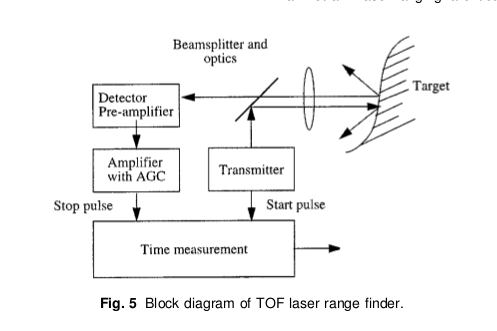
\includegraphics[width=\textwidth]{figures/raycasting/block_diagram.png}
    \caption{\textbf{CHANGE TO TIKZ} Block diagram of \gls{tof} laser range finder\label{fig:lidar_block_diagram}}
\end{figure}
A wide variety of lasers are used depending on the intended measurments range.
In the spacecraft case, laser providing peak energy in the range of \SI{15}{\mega\joule} are often required to measure distance of over \SI{50}{\kilo\meter}~\cite{berry2013}.

The laser range finder is frequently equipped with angle encoders to enable the definition of the position of the measurement point with respect to the sensor. 
Mechanical scanning is performed using a control system which  either move the entire laser range finder or only the measuring beam.
Focal plane scanning is another approach which reduces the mechanical complexity of a mechanical scanning system.
The laser energy illuminates the entire field of view on the surface.
An array of detectors are aranged to view the surface.
Each detector only views a portion of the total field of view and the signals are analyzed in the time domain.
Using this methodology, the system can simulataneously measure distance in multiple directions without any moving parts~\cite{amann2001}.

\subsection{Asteroid Mapping Operations}

Precise relative navigation and landing near asteroids is critically dependent on an accurate knowledge of the shape of the body.
The fine topological structure of the surface is not possible without a spacecraft in the vicinity of the asteroid.
From ground  based measurments, such as radar or optical telescopes, it is only possible to achieve a coarse model of asteroid, such as a triaxial ellipsoid representation~\cite{hudson1994}.
The size and shape of asteroid presents critical information into the thermal and collisional histories and more critically into their internal structure~\cite{cole1998}.

Typical missions spend months after arrival at an asteorid mapping and measuring the surface.
During this mapping phase, which requires upwards of \num{6} months, the spacecraft must maintain a specific trajectory and attitude to ensure best measurements of the surface~\cite{cheng2002,barnouin-jha2008}.
Both the spacecraft orbit and it's attitude is constrained to best satsify the competing requirements of the range measurements, spacecraft power, and Earth based communications.
These measurements are then sent back to Earth, and combined with the spacecraft orbit determination to simulateously estimate the asteroid shape, mass, gravity field, spin state, and spacecraft state.

Look at miller2002 for more detail and discuss that here

% TODO Discuss how the shape of an asteroid is determined in pracice currently
\begin{itemize}
    \item Talk about ground based imaging and citations (radar/optical)
    \item tlak about best knowledge of asteroid before arrival is a ellipsoid model (first mometn)
    \item Talk about sending missions to asteroids with laser altimeters
    \item Months of mapping and ground based OD
\end{itemize}

\section{Computational Geometry}

This section can discuss some background in computational geometry.

The majority of computational geometry algorithms are developed for simple planar \glspl{polygon}.

The surface of an object is described as the union of the surfaces of the polygons which define it.


\subsection{Surface Reconstruction}
One of the main mission objectives for asteroid operations is to generate the three-dimensional shape of an asteroid.
This shape generation is a subset of a larger class of methods called surface reconstruction.
The goal of surface reconstruction is stated as follows: Given a set of sample points \( X\) assumed to lie on /near the surface \( U \), create a surface model \( S \) approximating \( U \).
Surface reconstruction is a well-researched field and widely applied in the industrial and computer vision fields.
The generation of a surface from an object is important in reverse engineering, product design and medical product construction~\cite{amenta2001}.
The surface reconstruction problem is applied in a variety of fields in science and engineering including 3D scanning, surface reconstruction from contours and surface sketching~\cite{hoppe1992}.

Surface reconstruction, or sometimes referred to as 3D scanning, is the generation of accurate models of real world objects.
Surface Reconstruction techniques are frequently used to digitize sculptures/architecture, machine parts, archaeological artifacts, or terrain.
There are a variety of methods to digitize objects, such as laser range finding, mechanical touch probes, or computer vision techniques, i.e. depth from stereo.
From these digitization methods, a large collection, often times on the order of \( 10^6 - 10^9\), of points are generated.
From this \gls{point_cloud}, the goal is to construct a surface representation which is faithful to the original data, and the underlying object of interest.
This process of generating the surface should ideally have the following properties:
\begin{itemize}
    \item Fast - low computational cost
    \item Low memory - storing/operating on large collection of points is frequently memory constrained. Also for use in constrained enviornments
    \item Robustness - Algorithm must be robust to holes, noisy data, varying or low sample density
    \item Accuracy - the method should approximate the shape based on the data rather than interpolating between data points
    \item Features - ability to capture sharp edges or features
\end{itemize}

% TODO Describe different methods of surface reconstruction

The \gls{implicit_shape} representation allows for a complex shape to be defined by a single equation.
This approach has the additional benefit of unifying both the surface and volume rendering to a single equation.
The main advantage associated with implicit surface approach is handling sparse or scattered data.
It is possible to repair or edit the shape using standard implicit modeling operations.
For example, given two implicit surfaces
\begin{align*}
    F_1(x, y, z) &= 0, \\
    F_2(x, y, z) &= 0 ,
\end{align*}
one can define a new surface as
\begin{align*}
    F(x, y, z) = \mu F_1(x, y, z) + (1-\mu) F_2(x,y,z) = 0,
\end{align*}
where \( \mu \in \bracket{0, 1}\) is a design parameters defining the blending between the two input surfaces.
This blending allows one to use primitive shapes/models to create complex surfaces.
% TODO Find citation for this (blending of implicit shapes)
However, this implicit representation makes it difficult to modify the local shape of the surface. 
Examples of this approach include~\cite{bolitho2009,hoppe1992,ohtake2005}.
% TODO Describe in more detail the difference, drawbacks/advantages, of each implicit surface approach.

Surface reconstruction was first addressed in the early 80's~\cite{uselton1983,uselton1981}.
The main goal of this early work was focused on developing methods to accurately and efficiently display three dimensional data on a computing system.
The resulting work developed a computational algorithm to construct the three-dimensional polygonal representation of an object from the collection of points describing the surface.
The determination of a polygonal surface through a series of points is a relatively straightforward problem, as there an infinite number of solutions.
However, determining the ``best'' surface is a more challenging problem.
As the original surface is typically not available, hence the need for measurement and digitization, the quality of the resulting surface must be computed using the measurement points.

Another approach is to use the sculpting of delauney triangulation~\cite{boissonnat1984}.
Further refinements came with the notion of \( \alpha \) shapes~\cite{edelsbrunner1994}.
The notion of a signed distance function and the implicit shape representation proposed~\cite{hoppe1992}.
A modification of this approach extended it to a voxel grid~\cite{curless1996}.
Ball pivoting allows for a relatively simple method of determining the surface~\cite{bernardini1999}.
Next, another method seeks to project sample points, with neighbors onto a plane then lift the local two dimensional delauney triangulation to reconstruct the surface~\cite{gopi2000}.

Our overarching goal for the surface reconstruction is to develop an efficient algorithm which allows for online, or near realtime, surface reconstruction from a sparse point cloud.
Furthermore, this method should allow for an incremental update given a new partial point cloud.
For example, given an initial coarse point cloud representing the initial guess of the surface, new, high density data, is acquired in a specific location on the surface.
Instead of processing the entire point cloud, and recomputing the global mesh, an incremental update would allow for modification of only the local neighborhood of the additional data.
Another useful requirment would be the ability to easily combine two overlapping point clouds into a single surface mesh.
Finally, the resulting surface should be topologically valid and without holes, i.e. a polyhedron mesh with triangular facets.

\subsubsection{Watertight surface mesh}

There are two main approaches to generate water tight surface meshes.
The powercrust algorithm seeks to approximate the \gls{MAT} of a three-dimensional object~\cite{amenta2001}.
Then the inverse map is used to produce a watertight boundary.

Another approach is the tight cocone algorithm~\cite{dey2006}.
This reduced the complexity of powercrust and uses a post processing method to fill any holes.

\subsubsection{3D Scanning}
There are several different approches to acquire shape information of an object.
The computer vision field several approaches exist to determine the shape of an object.
In feature correspondance, landmarks are registered and compared across several different  views of an object. 
The shape of the surface is inferred given the known motion of the camera system~\cite{szeliski2010}.
Another approach is based on the different surface reflectivity of the surface, called shape from shading~\cite{szeliski2010}.

% TODO Mechanical scanning using a probe or laser scanner 
% TODO Range images are generated with distances to the surface. Assume known motion of camera (SLAM) if not known

In 
% TODO Talk about how we construct a mesh given a point cloud
\begin{itemize}
    \item Review surface reconstruction algorithms
    \item Talk about the one that is implemented inside VTK Hoppe papers
    \item 
\end{itemize}

\section{Updating a mesh}

In order to update a mesh given a single new data point, \( p \in \R^3\) requires the following steps:
\begin{enumerate}
    \item Determine the distance from \( p \) to the primitives of the surface
        \begin{itemize}
            \item This involves determining the distance to all the vertices, edges, and faces of the surface
        \end{itemize}
    \item Find the minimum distance to the primitives
    \item Based on the closest primitive decide on a method to incorporate \( p \)
        \begin{itemize}
            \item This step is still TBD, but the basic idea is to modify the connected edges/faces to incorporate \( p\).
                This will most likely require some form of Delauney Triangulation
        \end{itemize}
    \item Return the new mesh
\end{enumerate}

\section{Testing and Robustness}

\begin{itemize}
    \item Handle situation where no face/edge are in ``view''
    \item \( p \) is inside the surface
    \item \( p \) is on the surface, face or edge, or even a vertex
    \item Multiple primitives are equidistant from \( p \)
\end{itemize}

\section{Current Progress}

I've created methods to determine the minimum distance to the vertices, edges, and the faces of a mesh. 
The basic algorithm for each is shown below.
The computation of the closest vertex is fairly straightforward. 
However, the closest edge/face is less straightforward.


\subsection{Our approach}

Model LIDAR

Simulate measurements

Update shape

Update gravity model

Control based on new estimate of shape
